\documentclass[mres]{ucl_thesis}
%twoside for double page printing
\usepackage{graphics}
\usepackage{graphicx}
\usepackage{setspace}
\usepackage{epsfig}
\usepackage{subfigure}
%\renewcommand{\familydefault}{\sfdefault}
%\usepackage{palatino}
%\usepackage{lmodern}
%\fontsize{20}{24}\selectfont



\title{Using Congestion Exposure for Traffic Engineering}
\author{Imad GRANDI}

%\renewcommand{\baselinestretch}{1.5}
%\renewcommand{\bibname}{References}

\bibliographystyle{alpha}

\begin{document}
\maketitle

\clearpage
\clearpage
\fontsize{12}{15}
\selectfont
\begin{center}
\textbf{}
\end{center}
\clearpage
\begin{center}
\textbf{To my family}
\end{center}

\begin{abstract}
If I knew my thesis, I would know my abstract and guess what? It
would be HERE.
\end{abstract}


\begin{acknowledgements}
Words comprising the acknowledgements.
\end{acknowledgements}



\setcounter{tocdepth}{2}
\tableofcontents
\listoffigures
%\listoftables

\cleardoublepage

\chapter{Conclusions and future work}
\label{chap:conclusion}




\chapter{Conclusions and future work}
\label{chap:conclusion}




\section{Traffic Engineering}


Network traffic engineering is an old discipline in the telecommunication industry and has evolved with certain specificities for different networks types. This overview focus on the issues and techniques related to Internet and IP networks Traffic Engineering, yet many of these concepts are valid for other network contexts.

\subsection{Definition and problem description}
Traffic engineering is the discipline concerned with the performance evaluation  and optimization of  networks.  This aspect of network engineering applies technology and scientific principles to measure, model and control the traffic.  \cite {RFC3272}.  

The main objective behind this intervention is to enhance the network efficiency, as it is perceived  from both  traffic and  resources views. The first one is usually referred to as traffic oriented, and is concerned with the enhancement of the quality of service (QoS) parameters as seen by traffic flows. Including : minimization of delay, minimization of packet loss and maximization of the throughput. In particular, the aim of this project as mentioned above, will be the minimization of loss rate as the main objective of our traffic engineering protocol.

Meanwhile, the second category of policies said resource oriented,  deals instead with the aspect related to the optimization of the resource utilization. In fact, having some subsets of the network being over-utilized while others are underutilized is an indication of a network not being used optimally. Maximum path utilization is usually used in this context as the principle evaluation measurement for network performance. TEXCP (see 2.1.4), the protocol that we'll be comparing with the results of our own architecture is an example of such approach. 

But the question that many might ask is how much TE could enhance the network efficiency? And does it really bring a significant added value? Doubts about TE utility usually use the tremendous increase of equipments capacity to promote that the demand on the network could be answered by simply putting more capacity on the network and that it won't significantly increase the network operator bill since marginals cost are converging to effectively zero. However, this vision of the Internet is simplistic. Internet has evolved from a simple network for the research community to a sophisticated communication infrastructure that provides a rich panel of services. The new users of Internet can't settle any more for the range of best  effort services that the network offered initially. Network operators need to make sure that their customers are receiving the service they are requiring, and that they are able to differentiate the charging according to  these requirements. Moreover, the near deployment of  optical fibers and the increase of users expectation will mean that there will be more demand on the operator core network. The efficiency boost that TE could bring will help the operators to keep their margin. This is especially crucial in open market where fierce competition is taking place. The global context of convergence is taking down the incomes of classical operators, and the only way to keep a profit margin is by reducing cost and take the most from network their key asset. This is what Traffic Engineering attempts to achieve.

\subsection{Basic Concepts}

\subparagraph{TE as a controllability problem }:
\\Independently from the optimization policy approach, a set of control tools and mechanisms are usually invoked in order to accomplish this policy. These control actions could be divided in three categories: 

Acting on {\bf traffic management} parameters is used police aggressive users or to support services with differentiated Quality of Service. This could be achieved by using techniques like queue management, differentiated scheduling and traffic policing and shaping.

Acting on {\bf resources attributes and constraints} that include controlling link bandwidth, buffers etc.
 
Modification of {\bf routing parameters} to control how traffic steers within the network. 

\subparagraph{Routing and Traffic Engineering }:
\\This last category is particularly important in this project since it is primarily involved in taking advantage of path diversity within a network. The Internet hourglass implies that network should be kept simple with routing is the key provided function. The routing process involves core network nodes or routers to choose the path over which to send packets. One of the Internet design principle  for the network is that it should be kept plane and without any central nodes that might introduce  vulnerability. This means that routing protocol have as a requirement allowing the routers to take local decisions while ensuring consistency and packet being delivered to their destinations. Routing protocol like RIP and OSPF succeed in this purpose. However, the topology driven nature of these protocols implies that they optimise the path choice of each destination independently without considering the traffic demand on the network.  A solution that allows to go around these limitations could be achieved solution by manipulating configuration parameters of the previous routing protocols to enhance network performance.  In particular, by having an estimation of the traffic demand on the network, network management could choose the link weights  used by OSPF for example, on a way that results in an optimized distribution of traffic over the network could be achieved. In \cite{fortz00} an iterative algorithm is describe to optimise the network utilization by adjusting the weight through the use of heuristic mechanisms. This solution presents many advantages like compatibility with existing routing protocols and stability. In the other hand weight update frequency should be kept low since during updates routing consistency is not ensured.

\subparagraph{Traffic Engineering in MPLS networks}:
\\Routing restrictions are one of the difficulties encountered with traditional IP networks. MPLS  Multi Protocol Label Switching answers some of them by using a connection-oriented switching mechanism:  At the edge of an MPLS domain, the ingress LSR (Label Switching Router) adds a header to the packet and forwards it (see figure \ref{fig:mpls-header}). The label field in the header indicates to which FEC (Forwarding Equivalence Class) the packet belongs so core LSRs knows how to process it (in case of differentiated service) and where to send it next. 

\begin{figure}[h]
 \begin{center}

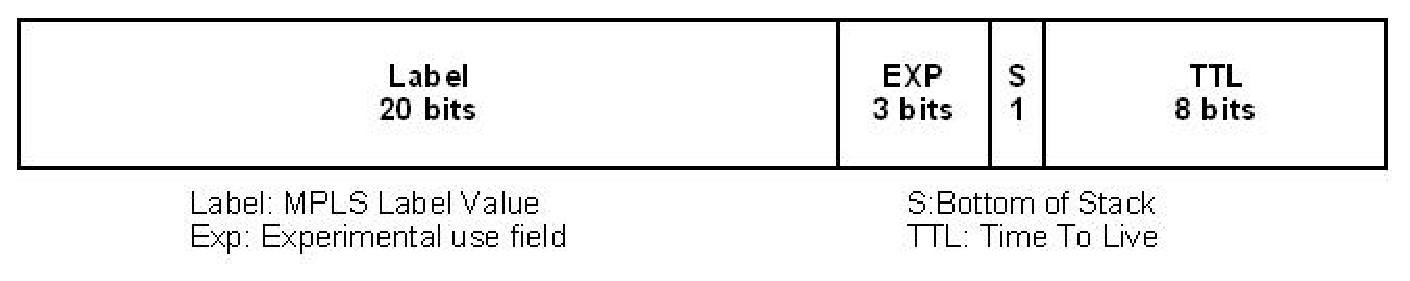
\epsfig{file=img/sec-2-1/1, width=4.5in}
\caption{
   The format of the MPLS header.

    \label{fig:mpls-header}
}
\end{center}
\end{figure}

MPLS allows the network management to provision tunnels within the network by configuring the core LSR. Edge LSRs are also configured to how they should assigned incoming  traffic to these tunnels. This open the way for new Traffic Engineering capabilities. After gathering information about the traffic, the network management configures tunnels and assign the traffic to them in a way that ensures efficient bandwidth utilization. As a result, Constraint-Based Routing that assign traffic to paths according to their bandwidth requirement could be achieved. For example this could be coupled with the Shortest Path First algorithm by simply removing from the network topology the links that doesn't satisfy the bandwidth requirement. Greedy heuristic is an example how the network management could proceed to assign routes to traffic. In this algorithm the flows in the network are aggregated in a decreasing order of bandwidth. The previous CBR algorithm is applied to the first flow on the list, and a tunnel is created in the network according to the result of this step. The network graph is updated and the process is repeated for the next flow in the list. Fairness is not ensured by this algorithm since the flows with the lowest requirement in bandwidth might end up not served.
\begin{figure}[h]
 \begin{center}

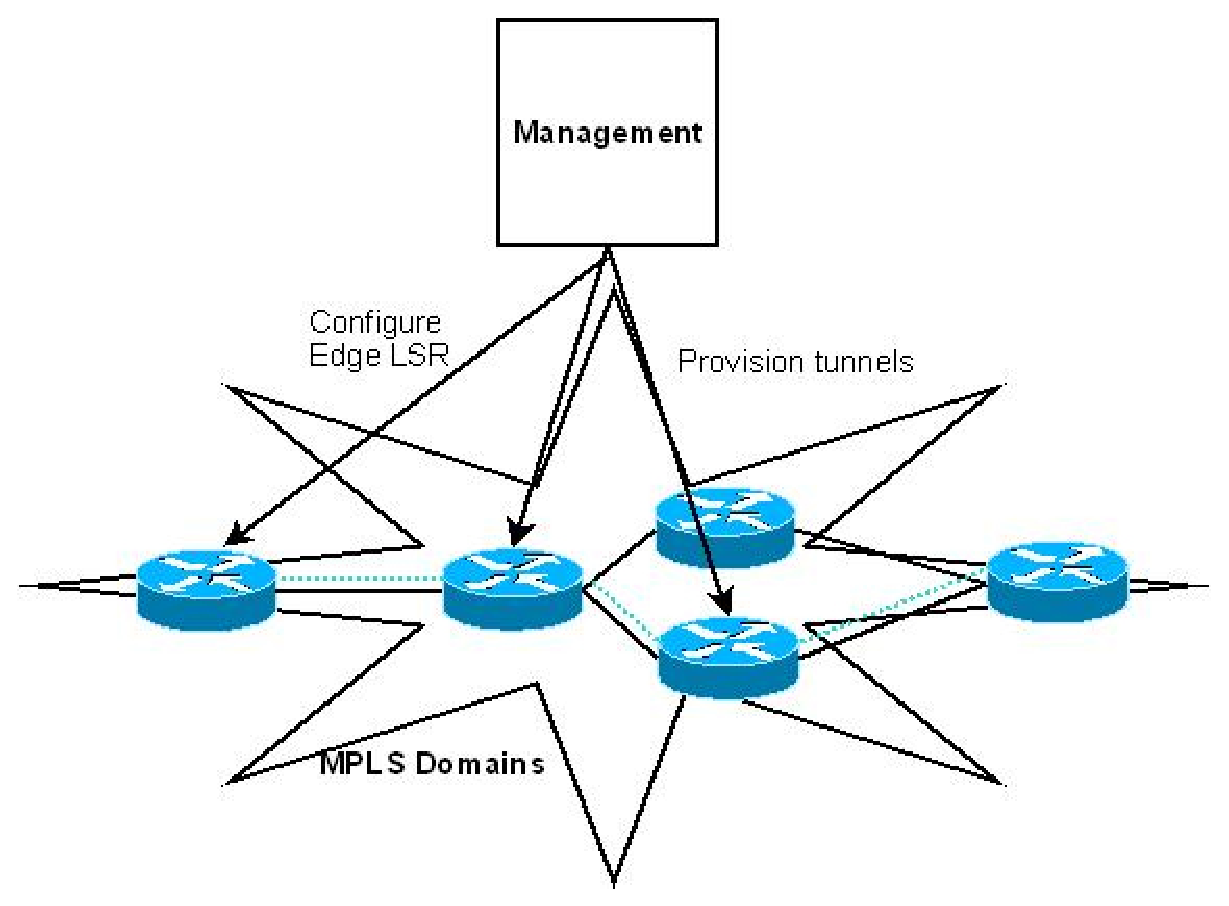
\epsfig{file=img/sec-2-1/TE2, width=4.5in}
\caption{
   Configuration of tunnels and control admission in MPLS networks.
    \label{fig:mpls-header}
}
\end{center}
\end{figure}


\subsection{Limitations}
	In both Traffic Engineering approaches, IP based and CBR in MPLS, the optimization of the routing is carried out for an estimation of the future demand based on long term measurement of the current traffic and expectation of evolution.  This is why both mechanisms are referred to as offline solution and raises some limitations. Indeed, actual traffic might differ from the network estimation and hence the routing might result in suboptimal or even inadequate distribution of the traffic on the network. Attacks, changes on external routing and link failures are frequent events and affect the traffic demands on the network. Failures are particularly wake point for this approach of routing. Offline TE deals with network failures by pre-computing alternatives routes. However, this could be done only for a limited set of network failures and TE should look for reroutes that perform relatively for a range of failures. As a result, suboptimal utilization of the network is frequent. Online TE is necessary to ensure that the network adapts in real time to changes on the demand.
	
A second characteristic of the previous approaches is that they require a global vision of the network to choose the configuration parameters. Some constraints are related to this property, like the scalability of the solution and the frequency of the update of the parameters. In distributive schemes, most of the decisions are made locally without requiring frequent interventions from a  central entity. 
In the next section, an example of a new TE solution that mitigate some of the limitation described above.

\subsection{Example of an adaptive traffic engineering protocol: TEXCP }

TEXCP is a a dynamic and distributed TE protocol that targets the optimization of network utilization. The basic idea behind TEXCP is that using path diversity we could balance the load among available paths in a way that optimizes utilization performance within a network. It is not itself a routing protocol but it sets on the top of existing MPLS systems and control how the flows are distributed over the network.

TEXCP is an online mechanism, meaning that it reacts to the changes on the traffic demands and potential network failures. It is distributed and doesn't necessitate an oracle that have a global vision of the network, boosting though its capability to scale in large networks. But, most importantly TEXCP has proved a strong stability that lacked most of the dynamic TE solutions until now. 
It targets performance optimization within a single domain, though it is considered as an Inter-Domain TE method. To have a more concrete idea, let's consider the simple architecture in (\ref{fig:texcp1}) :
\begin{figure}[h]
 \begin{center}

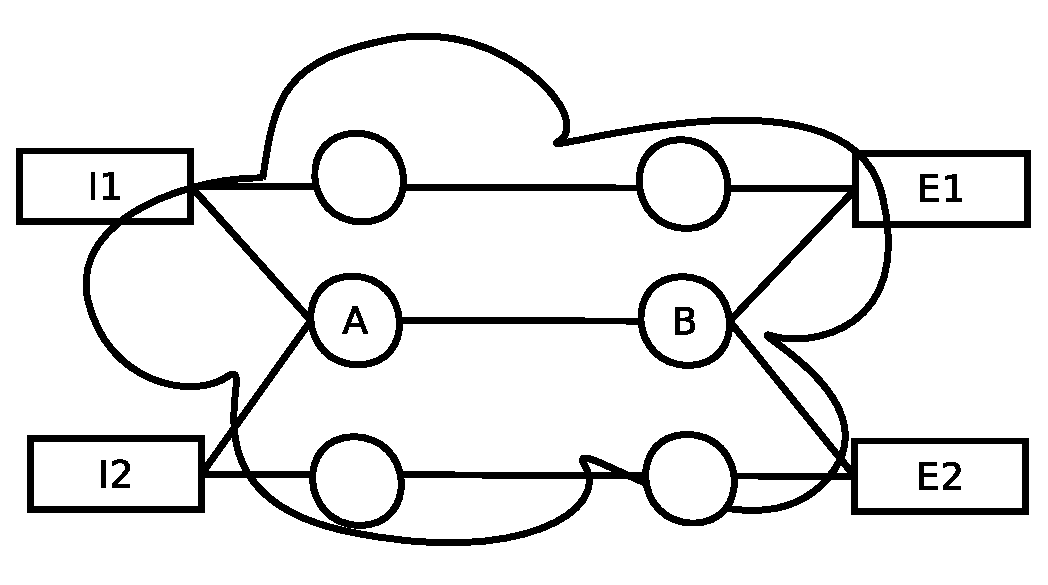
\epsfig{file=img/sec-2-1/TEXCPArchitecture, width=4.5in}
\caption{
   A simple architecture of an ISP network.
    \label{fig:texcp1}
}
\end{center}
\end{figure}
\\ From the ISP perspective, a flow enter the domain in an Ingress point (For instance I1) and leaves it in an egress point (E1 for instance). For this Ingress/Egress IE pair, two paths are available. In MPLS, as we've seen in the previous section, every packet arriving at the  domain will have a label allocated with the path it should takes. The path is chosen to meet a load balancing target : this load balancer called an agent will be associated to each IE pair and has as a target to balance the traffic among the preselected paths. The agent is also responsible of continuously probing the state of the network to feed the balancer with path utilization info. The probing mechanism is also used by the core routers to prevent oscillation and control the congestion.

{\bf Probing Network State}
\\ TEXCP load balancer needs to keep a track of the utilization state for each of the available paths. Hence the agent has to send a probe over all the available paths of  the IE pair associated to.  This probe will be processed by every router on the path until reaching the egress point, that will send back an acknowledgement message directly to the ingress. The format of the probe is shown in figure \ref{fig:texcp2}
\begin{figure}[h]
 \begin{center}
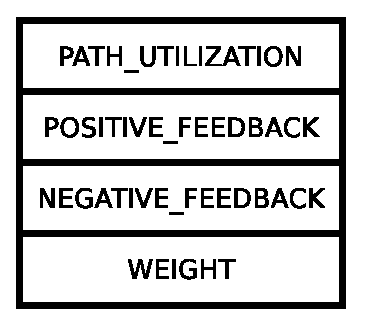
\epsfig{file=img/sec-2-1/TEXCPProbe, width=2in}
\caption{
   A simple architecture of an ISP network.
    \label{fig:texcp2}
}
\end{center}
\end{figure}
\\ The separation interval $T_p$ between two consecutive probes should be larger than the maximum round trip time RTT. However, the smaller is this value the faster the algorithm will converge. And hence it should be chosen slightly larger than RTT, A typical value for an average network is 100ms. During network congestion periods, it is possible that the probe get lost.

{\bf The Load balancer}
\\ As mentioned previously, TEXCP objective is minimizing the utilization in the network. Let's try to put this problem in a more formal way. Let $s$ an IE pair, and $P_s$ the set of selected paths for pair $s$. If $x_{sp}$ denotes the positive fraction of IE pair s traffic that goes through path p, the load balancer problem is to find the $(x_sp)$ configuration that will minimize the maximum utilization over all the network links 
\begin{equation}
\min_{x_{sp}} max_{l \in L} u_{l}
\end{equation}
subject to the following conditions:
\begin{equation}
u_l = \sum_{s} \sum_{p \in P / l \in p} \frac {x_{sp} }{C_l}
\end{equation}
\begin{equation}
\sum_{p \in P_{s}} x_{sp} = 1,  \forall s
\end{equation}
\\ This could be achieved if every agent tried to equalize the loss that it sees over all the controlled paths. According to the path utilization and the current rate distribution, the agent will send more traffic on underutilized paths and less traffic on over-utilized ones. This amount is calculated according to:
\begin{equation}
\Delta x_{sp} = \frac{r_{sp}} {\sum r_{sp'}}  (u' - u_{sp}) 
\end{equation}
where $u'$ the average path utilization. For the path with the minmum utilization a small positive factor is added to avoid that the oath with current small rate stop being used. The new value is path ratio could be calculated as the equation bellow then normalized :
\begin{equation}
x_{sp} = max(0, x_{sp} + \Delta x_{sp}
\end{equation}

{\bf Feedback}
\\Due to the distributed nature of TEXCP, instability and oscillation may occurs. Let's consider again the simplified architecture in figure \ref{fig:texcp1}. Link AB, is shared between pair I1E1 and pair I2E2 and hence in the case where the link is underutilized, agents associated with both pair will react by sending more traffic over this link and potentially causing the link to be over-utilized. Hence, it is necessary to have a feedback mechanism that will allow the core nodes -in particular node A-  to control and synchronize the answer of the multiple TEXCP agents that use the link. This mechanism is similar to what is used for congestion control when multiple sources sharing the same bottleneck attempts to adjust their rate and end up causing the bottleneck utilization to oscillate. The solution for both problems is to explicitly inform the sources of how much they should increase or decrease their rate. In order to provide the sources with such information, every core router needs first to update the aggregate feedback every $T_{p}$ seconds and then include within the probe. The aggregate feedback is an upper bound of how much the global traffic sent to the link should increase/decrease. Hence, the aggregate feedback is positively proportional to the spare bandwidth S (S = capacity -load) over the link and the negatively to the current buffer size Q.
\begin {equation}
\phi = \alpha . T_{p} . S - \beta . Q
\end {equation}
The next step is to divide this aggregate feedback over the available sources, TEXCP adopt a Max-Min allocation policy to divide this aggregate feedback, and hence installing a fairness that will prevent congested IE pairs from starving the others. Additive Increase Multiplicative Decrease (AIMD) standard is used to achieve this fairness and hence: 
\begin {eqnarray}
\Phi \ge 0 \Rightarrow \delta^+ = \frac{\Phi} {N}, \delta^- = 0 \\
\Phi \ge 0 \Rightarrow \delta^+ = 0 , \delta^- = \frac{\Phi} \phi_l
\end {eqnarray}
Where N denotes the number of active IE pairs that the router is seeing, and $\phi_l$ is the aggregate load on link l.

Before continuing on how this information is sent back to the IE agents, we would like to turn the reader attention to the scenario where multiple solutions of the optimization problem exist: consider a simple example where the two IE pairs in figure ?? have the same traffic, and and that the two links have the same capacity. One solution is that each router send one half of its traffic over each link, while the second solution is that the the first pair send all its traffic in link 1 while the other pair use the other link. In both solution the network utilization is the same and optimal, however the second solution has the merit of a reduce delay. So it we be good in case where multiple solution exist, shortest path are prioritized. This condition could be implement through the use of a weighted fairness allocation of the aggregate feedback 
When the ingress router send the probe, the fields will be updated by each router as:\\
\begin{eqnarray}
PATH-UTILIZATION = max (PATH-UTILIZATION, ul ) \\
POSITIVE-FEEDBACK = min (POSITIVE-FEEDBACK, \delta^+ ) \\
NEGATIVE-FEEDBACK = max (NEGATIVE-FEEDBACK, \delta^− ) 
\end{eqnarray}
Once the probe reaches the egress router, the router send back directly the final values. The first field in the probe is the utilization of the most congested path and in a similar way, the value for the feedback. The agent will update his sending rate $g_sp$ according to AIMD :
\begin{equation}
g_{sp} = g_{sp} + \delta^+ - g_{sp} \cdot \delta^-.
\end{equation}

\subsection{Splitting the traffic : FLARE}

\\ What the agent needs to do is to update $(x_{sp})$ the splitting ratio of the incoming traffic over the available paths. Traditionally, traffic splitting was tackled from two approaches. The first one is packet-based. However, this solution is very harmful to transport protocol that are sensitive to packet reordering like TCP. The second solution to split in flow basis, i.e. all packet of the same flows are sent over the same path. By assuring that a flow's packets goes over the same path, packet reordering won't take place and hence TCP could achieve a better performance. However, the flows have different sizes and characteristics hence this approach of traffic splitting deviates usually from the desired splitting ratio. An intermediate solution is described in \cite {sin1}, that take advantage from TCP burtsiness to do the splitting. A TCP flow life cycle is divided into a set of packets bursts called flowlet separated by idle periods. The flow-lets could be characterized by the minimum time that separate two successive flowlets. If we rightly choose this value larger then the value of delay difference , we could send the packets of the different flowlets in different paths without risking reordering problems: Let's consider a simple scenario where the last packet of a flowlet leaves the paths divvergence points at time $t_0$. If we know that the when the 
FLARE suggest also a splitting mechanism that uses a Token-counting algorithm, 
The final algorithm could be sum up in the following 3 steps:

1-when a packet arrives the counters of all the flows are updated as follows:
\begin{equation}
c_{sp} = c{sp} + x_{sp} \cdot PacketSize.
\end{equation}

2- if the packet flow is not TCP or the last time the flow has been seen is older then the time out value, the packet is sent on a the path with the highest token counter value. The packet is sent over the same path as the last packet of the flowlet.\\

3-The last seen time is upadated as wel as the counter of the selectedpath according to :
\begin{equation}
c_{sp} = c{sp} - PacketSize.
\end{equation}

\section{Congestion Control in Internet networks}
\subsection{Problem description}
A key characteristic of IP networks is their packet switching mechanism that allows a significant increase in the efficiency of bandwidth utilization. This efficiency is explained by the fact that multiple communications could take place over the same physical resource. However, this scheme rises the important question of how the capacity should be shared. And Internet discovered this in the hard way; during the mid 80' a serial of network crashes took place: high packet delay, high loss rate and  low  goodputs are the characteristics of the communications taking place then. These are now the symptoms of a network being over-utilized, and though these collapses had been baptised as Congestion Collapses \cite{RFC896}. 

As described in the RFC, the causes of this problems is that the offered load in the network is over passing the network capacity resulting in full queues and so increase delay and more packets being drop. The same RFC state that the problem particularly occurs when TCP is the transport layer being used over IP. Rightly, TCP retransmission mechanism was really clumsy. Indeed, when the liable transport layer considers that a packet wasn't routed to destination it retransmits not only one but multiple packets. This means additional load over the already congested network and congestion getting worst. But even if this retransmission scheme was replaced, it is up to the end host to adapt their transmission rate to limit the congestion and enhance the overall network performance. This is what was achieved through the implementation of congestion avoidance algorithm proposed by Van Jacobson [Jacobson88] for TCP. The same report suggested also that the network performing congestion control might enhance further the global performance. Some of the techniques used by the network were introduced later in what is known today as Active Queue Management AQM.
\subsection{TCP and congestion control algorithm}
Transmission Control Protocol TCP is a transport layer protocol that provides a connection-oriented, reliable stream delivery service over the connectionless unreliable IP network. As a transport protocol it provides a demultiplexing function that allows several process or flows at a single IP address to communicate concurrently. It provides also reliability by establishing a connection with the destination end host, so data is transferred and acknowledge in terms of byte streams enabling thus the possibility of retransmissions when the losses are detected either by the expiration of the acknowledgement timer or the reception of acknowledgement of previously acknowledged bytes (duplicate acks).

 \begin{figure}[h]
  \begin{center}
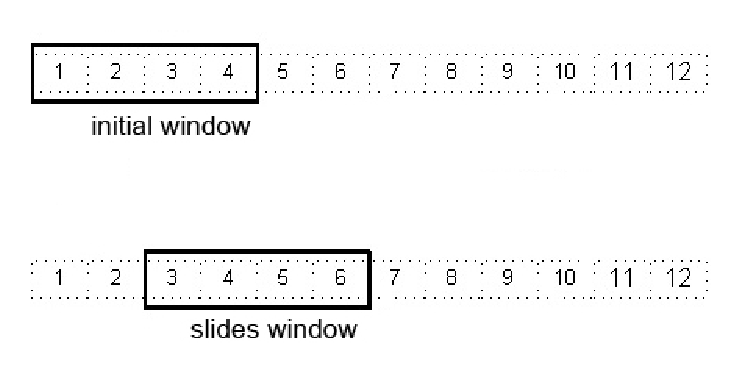
\epsfig{file=img/eps/CC1, width=4.5in}
\caption{
  The concept of sliding window.
    \label{fig:swnd}
}
 \end{center}
\end{figure}

To avoid bandwidth wastes that usually go with positive acknowledgement schemes, TCP use a sliding window algorithm that limits the number of segment a sender could transmit before receiving acknowledgements. Once the acknowledgement of the first packet arrives the window slides and a next packet could be sent. The number of packets that could be sent before receiving a first acknowledgement is called the window size(Figure\ref{swnd}). Thus, the transmission rate of a sender could be estimated in function of the window size as:
\begin{equation}
R_{Tx} = \frac{Window size}{RTT}
\end{equation}
Where RTT is the Round Trip Time which is the necessary time for the packet to arrive to the receiver and that the acknowledgement to get back. This window side is variable and limited by the receiver advertisement window, that allow the receiver to specify the number of bytes that it could receive, and also the congestion window that is used by the sender to limit the transmission rate to control the congestion. A variety of congestion control algorithms exist depending on TCP implementation but they all have “Slow Start” and “Congestion Avoidance” in common. 

 \begin{figure}[h]
  \begin{center}
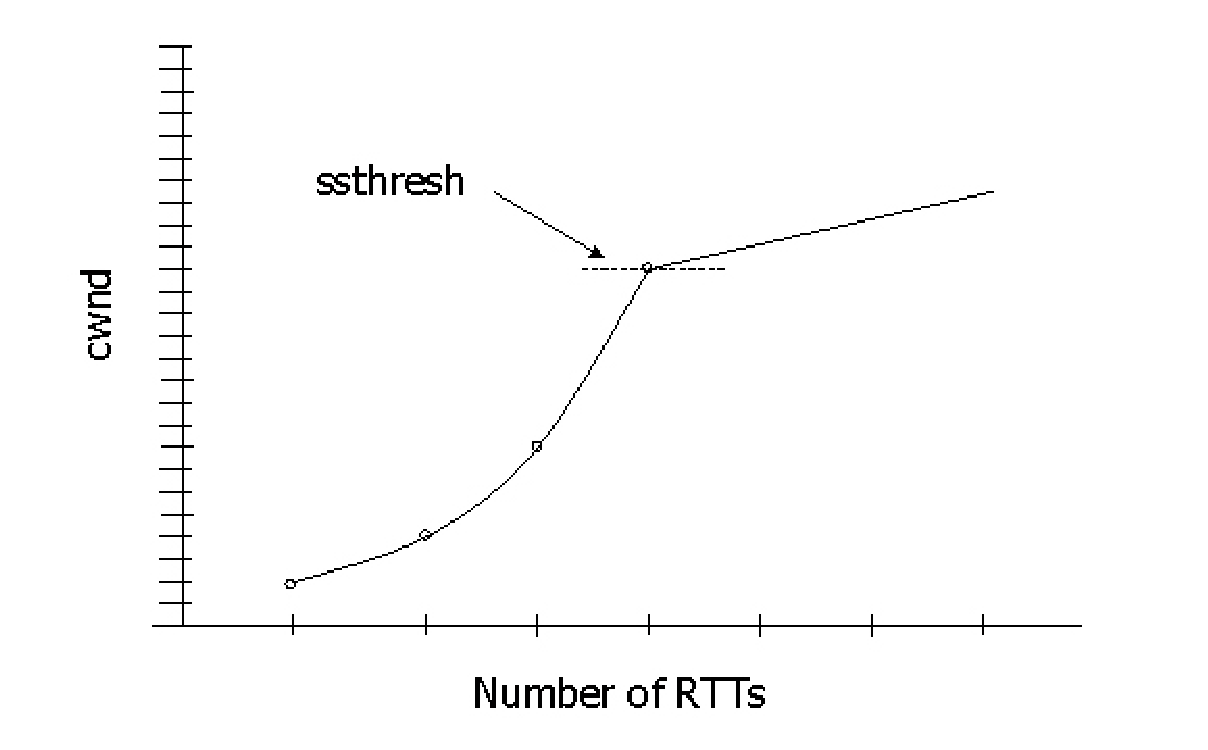
\epsfig{file=img/eps/CC2, width=4.5in}
\caption{
  Slow Start and Congestion Avoidance.
    \label{fig:SSCA}
}
 \end{center}
\end{figure}

So during the Slow Start phase the sender increase exponentially the congestion window {\it cwnd} until reaching the slow start threshold {\it ssthresh} then TCP sender enters the “Congestion Avoidance” phase where the cwnd is increased by 1 every time an acknowledgement is received.
TCP implementations differ on how to identify them (Retransmission TimeOut (RTO) or duplicate acks) and how to react to losses: either by reducing the cwnd to 1 and enter again the "Slow Start", or to ssthresh in the case of “Fast Transmit” and TCP transmitters enter directly the phase of  “Congestion Avoidance”. {\it ssthresh} is reduced also and usually put to the half of the cwnd before that the congestion occurs. Thus this algorithm is referred to as Additive Increase Multiplicative Decrease AIMD. It also associates TCP transmission rate to the loss ratio over the path. The association could be approximated through Mathis Formula:
\begin{equation}
R_{Tx in packets} \approx \frac{1}{RTT \cdot \rho}
\end{equation}

\subsection{Active Queue Management}

An individual action from the end hosts toward the congestion presents some limitation. End hosts are only aware of the congestion when the packets start being dropped and they react simultaneously to the congestion causing hence a global synchronization. [RFC 2309] states that using some queue management techniques for congestion control will allow the number of dropped packets to decrease and prevent global synchronization. 
RED or Random Early Discard is one of these scheme that consists on starting to discard packets randomly before the queue is completely full:

 \begin{figure}[h]
  \begin{center}
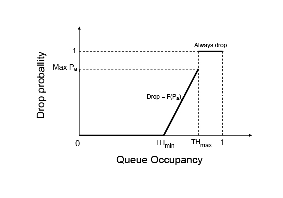
\epsfig{file=img/eps/CC3, width=4.5in}
\caption{
  Drop probabiliry in RED.
    \label{fig:RED}
}
 \end{center}
\end{figure}

The algorithm steps are the following:\\
1-If the queue size is smaller than $T_{min}$, packets are enqueued.\\
2-If queue size is larger than $T_{max}$ discard the packet.\\
3-If the queue size is between $T_{min}$ and $T_{max}$ packets are dropped according to a probability p.\\

The key to make the algorithm works is to well choose its parameters. Some of the consideration are to ensure a high utilization of the outgoing link and provision enough difference between $T_{min}$ and $T_{max}$ so the end hosts are informed and could react. Also differential treatment could be applied by using different value of the discard probability p for different flow classes. 

{\bf Explicit Congestion Notification (ECN)}
\\RED could also be combined with ECN [RFC 2481] another AQM technique that allows the network to explicitly inform the end user of the congestion instead of relying only on the host detecting packet losses. The network feedback is passed to the end user through two unused bits in the IP TOS byte. \\

\begin{center}
\begin{tabular}{| l | c| } \hline 
00 & Non ECN-Capable Transport - Non-ECT \\ \hline 
10 & ECN Capable Transport - ECT(0) \\ \hline 
01 & ECN Capable Transport - ECT(1) \\ \hline 
11 & Congestion Encountered - CE  \\ \hline 
\end{tabular}
\\
\caption{
  ECN codepoint.
    \label{fig:ECN}
}
\end{center}

\\ECT(0) and ECT(1) indicates that the originator of the packet is ECN capable and in this case, if the packet has experienced congestion the router will mark the packet with CE code point. It could be carried outusing the schem defined by RED and allows transport protocols and particularly TCP to be notified of congestion without having to experience loss. 
By marking packets instead of dropping them, ECN reduces the number of dropped packets. It also reduces the delay for the network layer to consider a packet as dropped and hence the delay of its reaction to the congestion. Finally, it is an in-band signaling mechanism and doesn't add additional traffic which is particularly useful when the network is experiencing congestion.





\section{Congestion Exposure and Re-Feedback Principles}
\subsection{Motivation}

As explained in the previous section, congestion control in TCP/IP networks is mostly based end users running congestion avoidance algorithm. In fact, every TCP routine increases its transmission rate until packets are dropped due to a congestion in bottlenecks. This mechanism might seems weird, but it is fundamental in the Internet architecture where there is no circuit dedicated for a communication and though no fixed rate. The second outcome of TCP congestion avoidance algorithm is capacity sharing. From a first glance at the mechanism , we might think that it could be considered as fair since all the users are  running the same algorithm and respond the same way to the state of the network. However, this fairness is only a mirage. A first way to walk around TCP limitation is by running simultaneously multiple TCP instance, since every instance gets an equal share of the available capacity. But, the real problem is that the users are not all the same, having different behaviours and participating differently to congestion. This problem is a real puzzle for ISPs today. A small part of their customers that uses greedy applications, like peer-to-peer and video streaming, are taking more and more shares of their network capacity \cite{RFC5594}.  Hence, they couldn't leave any more the capacity sharing task for TCP and they turned to new methods for controlling the traffic and explicitly making sure that heavy users are not taking the whole bandwidth. However, the success of these methods is mitigated because the lack of the information about the congestion a flow is causing and though they are unable to treat them according to what really matters. Hence, making congestion visible in the network layer is a necessity to build a fairer sharing mechanism. ECN(see section ??), the protocol that the core routers uses to explicitly inform the end hosts of the congestion they are causing is  a step in the right direction.  Using ECN, a network is able to calculate the congestions caused by the flows that a user receive. But this is not enough, the problem with P2P applications for example is the congestion that they users are making in their upload sense and also receiver could also ask “politely” the senders to change their rate and can't imply how they work,  congestion exposure goal is to make the congestion fully visible in both direction and for all the network nodes.

\subsection{Overview of  the current traffic control methods}
As pointed out in the previous section, ISPs are attempting to control their customers traffic. These methods could be divided in three categories: network layer measurement based, transport and application.

L3 Measurement policing

The original design of Internet supposes that routers looks only for information in the detained in the network layer. Two possible measurement could be carried on: volume and rate.

Volume accounting is the easiest information that a network provider could calculate to have a clue about who are heavy users . To obtain this information, it is enough to look for the packets sizes at the IP header and then add them up. ISPs could use this information to impose the maximum limit for a user in a period of time. However, volume accounting doesn't give a real vision of the damages that a volume of traffic is making since it might depends on the period of time as well as the part of the network where it goes.

The second tool in this category is the rate measurement. It is especially the case for the accounting between ISPs, where for instance the charging could be made on the percentage of peak rate crossing the border. A simple way to measure the rate is by accounting the volume for short periods of  time. Traffic shapers could be used to make sure that the traffic doesn't overflow the maximum rate. Even, if such policies will allow to limit the damage of heavy users on the others, but they induct situations where some users are allocated more capacity than they really need to prevent the risk of all the users sending fast at the same time, resulting though a poor bandwidth efficiency.

Higher Layer Discrimination

ISPs are aware of the limitation hourglass design of the Internet and in the same time the equipment capacity is increasing exponentially, and the reasons for keeping the routers simple are diminishing. Hence, some ISPs have introduced DPI operations that allow to investigate the packet to identify the flows that belongs to the applications that they thought being responsible for the network congestion. A common example is P2P file sharing. ISP regard these applications as ith low value for the customers and cause most of the congestion problems in the network. These technique are in the center of the ongoing debate about Net Neutrality. Even more, the efficiency of these techniques is being questionnaire since P2P applications 
responded to the DPI by using encryption techniques.

The last example is usually called bottleneck rate policing. They require the deployment of the rate policers at the bottleneck that based on some assumption over what an flows might accept about traffic shaping. Another problem with these approaches is that the traffic usually traverses multiple bottlenecks and therefore limiting hence the utility of the solution.

\subsection{Re-inserting the Feedback Re-Feedback}
All the approaches described above fail in controlling the traffic based on what counts the most, the congestion caused by the customer. The main reason behind this failure is in Internet design itself that doesn't provide enough information about congestion to the network. Re-Feedback attempts to correct the weak points in Internet feedback mechanism. As explained, previously, ECN markings  till routers about the congestion on the upstream route (the part of the route between the sender and receiver). Similar accounting could be achieved with the Time To Live (TTL) field. The modification that Re-Feedback is suggesting, is that instead of aligning the information at the source, the sender modifies the field by targeting to reach a certain metric at the destination. For example, TTL field shouldn't be initiated  to 255 at the source, but should be modified to reach an agreed value at the destination (say 16). This means that the routers by inspecting the IP header will be able to have an estimation of how many nodes left for the packet to reach destination.

Re-ECN is the implementation of this principle using ECN markings that will attempt to provide a metric for accounting the congestion. As table ?? depicts, a value is associated with each markings, for example a neutral packet has a value of 0 and if it experience congestion it will become negative with a value of -1, and the accounting at the routers is decremented. Thus, the sender should transmit enough packets with a positive value +1 (router increment their accounting when they see positive packets)so the accounting near the destination won't go bellow 0. If these packets experienced itself congestion they will be cancelled 0. Now the network needs to control the network at two critical points. At the egress where it could have a vision of the congestion for the full path, the operator should ensure that the source is putting enough credit or positive packets so the accounting stays positive, and provision incentives for that ( for instance dropping packets  where the metric is negative). Now the network is capable to account the congestion created by the source by accounting the positive packets that correspond to the congestion the source make. Based on this metric the network will be able to identify the sources that cause most of the congestion and could treat them accordingly. For instance, each source will be allocated a limit of the positive packets and once it over pass this limit the quality of the service might drop (traffic policing, limited bandwidth etc.)

\subsection{Use Cases}

Now that the operator is able to charge the customer on explicitly the congestion they are causing, Heavy users are motivated to act less aggressively when the network is experiencing congestion.  This won't significantly delayed their communication, since when “light” users acting more aggressively will have a bigger share allocated and they will finish their communication faster, so the heavy users could recuperate the whole bandwidth again. 

Other benefits could be drawn from the Congestion Exposure scheme like the use of the new encoding to identify the attacks by their patterns. And the aim of this project is to evaluate the use of another  congestion exposure scheme in Traffic Engineering.

\chapter{Conclusions and future work}
\label{chap:conclusion}



PREFLEX Path Re-feedback with Loss Exposure

This chapter introduces PREFLEX, a new architecture for pooling resources -more particularly path diversity- that promotes cooperation between end hosts and edge network and attempts to draw benefits from Congestion Exposure (see 2.3). Section 3.1 presents Loss EXposure LEX, a congestion exposure protocol that end hosts uses to reveal experienced losses to the network. While in section 3.2, we are going to see Path RE-Feedback PREF the second components of the architecture, that edge network uses to inform the end host of its path preference. This path preference is based on  the split that the balancing algorithm described in section 3.3 chooses to optimize the global congestion experienced in the different paths.

\section{Loss Exposure}

During the presentation of the Congestion Exposure concept, we've discussed how there is a lack of congestion information available at the network layer and how it affects the network efforts towards controlling the congestion and fairly charging the customers for the congestion that they are causing. This lack also affects the optimization process of networks, by restricting mostly their target to the optimization of resources utilization rather than targeting directly the quality of service customers are getting. Keeping the same line of thinking, Loss EXposure is a simple protocol that allows end hosts to signal path loss back to the network. The information about the loss traditionally confined in the transport layer will be revealed by explicitly marking the IP header of retransmitted  packets.

Establishing the feedback

End hosts need to establish a connection first, before the source begins signalling back the feedback it gets about the loss. The packets of this first exchange are marked with FNE code point. The resetting of  feedback loop takes place essentially during the creation of the transport layer end-to-end connection.  Hence packets marked with FNE corresponds to SYN and SYN-ACK messages in TCP terminology. But, the restart of the loop could also take place after a long idle period or new attempts for retransmission after successive timeouts.

Many advantages could be drawn from this signalling. First, it eliminates the network need for inspecting higher layer fields to identify connection establishment. But most of all, a new  association between the end hosts, and visible at the network layer, could be established using the FNE-marked packets. This association could be used by the middleboxes to allocate state for different functions like control admission and traffic shaping. This association similar to the network flowlet used in FLARE (see 2.1.4) for traffic splitting presents the same advantages since it allows to divide transport flows in a succession of packet streams of smaller granularity. However, it presents an additional advantage since both network and transport layer are aware of it and it could be used for the latter to explicitly express that it desires packets belonging to this stream to be routed all on the same path.

Code Point
Explanation/Meaning
Not-LECT
Not Loss Exposure Capable transport
LECT
Loss Exposure Capable transport
LEx
Loss Experienced
FNE
Feedback Not Established

Echoing the Loss

Now that the feedback has being established, the end host could start revealing to the network the loss experienced in the last period of time. LEX is a simple form of Congestion Exposure that requires the end host to only mark retransmitted packets with the (LEx) code point. For the rest of the non retransmitted packets, the (LECT) code point is used. Coupled with the ECN marking, the network is in possession of two signals of information: an end-to-end vision of the experienced losses by the end host over the path during the previous RTT thanks to LEX, and the  current congestion experience at the upstream of each node that ECN markings provide. Hence the network could estimate rest-of-path congestion. But mostly the network will be able to accurately estimate the end-to-end loss experienced in every path by simply dividing the number of bytes marked with (LEx) code point,  by the total number of bytes marked either LECT or LEx. As we are going to see in the balancing section, the information of the loss experienced in the different paths will be used to decide the amount of flows that will in every path. Another potential advantage that could be drawn from this marking is that the network could prioritize retransmitted packets.

Analysis of the LEX protocol and comparison with re-ECN

LEX reuses many of the concepts that the congestion exposure protocol re-ECN has brought. The use of FNE packets by the network for allocating the state is one example of the similarities. Also by coupling LEX with ECN markings the network will be able to estimate the rest-of-path congestion and hence a metric will be available for both charging the customers on the congestion that they are causing and evaluating the service offered by the network. However, the drawback of this scheme is that it requires the aggregation of the packet streams to be carried out close to the source while the policing should be placed close to the receiver. This is not a significant problem, since the focus of the PREFLEX is to allow stub domains to balance the congestion. Moreover, LEX and re-ECN could coexist together: LEX code points could be easily added to the re-ECN mechanism since three of them have equivalent code points in re-ECN while LEx could be attributed to the currently unused code point in re-ECN. Hence LEX could be a complement to re-ECN. Thus, LEX could be considered a bridge for re-ECN until congestion notification is widely deployed in the network.

\section{Path Re-Feedback}

The second component of the architecture is PREF mechanism that allows stub domains to inform the end host of its path preference, From one hand it allows end hosts to be aware of the path the packets are taking. It also provides another solution for the problem of traffic splitting (see 2.1.3), since end hosts knowing the network path preference could take in charge the responsibility of assigning packets to the path. Using FNE packets to divide the flows to smaller granularity permits to achieve an accurate splitting of the traffic while preventing end hosts to suffer from packet re-ordering. PREF uses incoming FNE packets to trigger the path selection process for outgoing paths. This means that receiver will be left with the freedom of deciding when it is best to request a new path. The efficiency of the scheme is dependent on the strategy adopted by the receiver for this matter. It also could be a source of vulnerability for the network since FNE packets requires from the network  additional resources, both computational -e.g selecting a path- or in memory -keeping a state-. Therefore, the network might need to provision mechanism to limit the FNE packets rate.

The implementation of the path re-feedback could take place in the DiffServ field of the IPv4 header and more precisely the bits reserved for local use. So, once the edge network re-feedback its path preference the end host should tag all the subsequent packets with the path value.
It is worthy to mention that eve if the two architecture components are functionally separate their cooperation is necessary to achieve the target of congestion balancing. In the next section we will see how the architecture manage to optimally balance the congestion over the available paths.

\section{Balancing by PREFLEX}

\subsection{Algorithm requirements}
The algorithm has as a key target to succeed in balancing the congestion equally over the available routes. To this optimization goal, the design of PREFLEX architecture implies some additional requirements: 

First, the path probing mechanism in PREFLEX relies on the loss experienced on the traffic that the end user sends over each path. Obviously, if  there is no traffic sent over the path there will be no feedback about the path congestion. Hence, the algorithm should attribute a minimum share of the traffic over all the paths,
The algorithm shouldn't make assumptions about the actual distribution of the flows based on the previous splits: since the path selection process is triggered by the receiver, the algorithm shouldn't expect that all the flows had have seen a new path assigned between two decision intervals. Only, the flows that had sent FNE packets will be distributed according to the last desired split, while the long living flows that didn't ask for a new path will keep their old path and thus their distribution is based on previous splits. The actual flowlets distribution is unknown and a combination of the two.

\subsection{Algorithm inputs and outputs}

PREFLEX balancing algorithm requires to keep some information about each of the available paths. These information are contained in the routing entries that are organized in tables for each egress destination $d$. The nature of this destination depends on the context were PREFLEX is invoked so it may correspond to a set of IP destinations addresses or prefixes, or it may correspond to effectively the  address of the egress gateway to reach an external domain in the case of intra domain Traffic Engineering. 

A set of available routes $P_{d}$ is associated with destination $d$. For each route $i$ from the previous set, a table count of LEX markings is kept. In particular, $L_{di}$ be the number of bytes marked with the loss experienced codepoint and sent through route $i$ in the previous time period and $T_{di}$ denotes the total number of accounted bytes on routes $i$ for the same period of time. 

The two inputs will be used by the algorithm to determine the split of destination $d$ traffic over its permitted routes. The split indicates $f_{di}$, the fraction of the flowlets to destination $d$ that should be assigned to path $i$. 

\subsection{Algorithm description}

The flowlet split for each destination could be calculated according to three approaches. An equalization mode where the tendency is to equally distribute the traffic over the flows, a conservative mode where the importance is given to the stability of the algorithm and to prevent overreacting for small fluctuations. And the last one is to balances the losses obviously.
Hence, the final split is obtained as the combination of the splits calculated according to the three tendencies:

\begin{equation}
f'_{i} = \beta_{E}f'(E)_{i} + \beta_{C}f'(C)_{i} + \beta_{L}f'(L)_{i}
\end{equation}

Using the dash notation for the same quantities in the next time period, where $f'(E)_{i}$, $f'(C)i_{i}$ and $f'(L)_{i}$ consecutively denotes the split calculated according to “equalization” approach $E$, “conservative” approach $C$, and “loss driven” approach $L$. Similarly, $\beta_{E}$, $\beta_{C}$ and $\beta_{L}$ denotes positive factors associated with each mode and that verifies $\beta_{E}+\beta_{C}+\beta_{L} = 1$. 

Now by definition $f'(E)_{i} = 1/N$. For the other two splits we need an additional assumption. As explained in 3.3.2,  the balancer doesn't necessary achieve the desired split by the next period of time. Hence the actual flow distribution will be estimated as $T_{di}/ T_{d}$, the fraction of bytes to destination $d$ that takes route $i$. $T_{d} = \sum_{i \in P_{d}}T_{di}$ denotes the total bytes for destination $d$,  and in a similar way let $L_{d} = \sum_{i \in P_{d}}L_{di}$ the total losses bytes for destination d. The accuracy of this assumption could be explained by the fact that flows experiencing the same loss rate will have equal transmission rates (Mathis formula).

Hence, for the “conservative” approach $f'(C)_{i} = T_{i}/T$. While for the “loss driven” approach we will choose the split as  $f'(L)_{i} = T'_{i}/T''$ so that the loss rate on the different routes is equal.

The loss ratio is defined as $\rho_{di} = L_{di}/T_{di}$ for all the permitted routes $i.$ The loss rate is an unknown function of $T_{i}$ and the link bandwidth $B_{i}$. However, it is reasonable to assume that the loss rate is increasing with $T_{i}$ and decreasing with $B_{i}$. Hence, what ever the true function is, we could assume that in a small region around the current values of $T_{i}$ and $B_{i}$, it is locally linear $\rho_{i} = k_{i}T_{i}/B_{i}$, where $k_{i}$ is an unknown constant. Substituting gives
\begin{equation}
B_{i}/k_{i} = T_{i}^{2}/L_{i}
\end{equation}

So for the next period of time, loss rate are $\rho'_{i} = T'_{i}/L'_{i} = k'_{i}T'{i}/B'{i}$. Hence, to make the loss rate equal for all routes, we should choose $T_{i}$ that verifies $L'_{i}/T'_{i}=C$, where C is an unknown constant. Therefore we should take  $T'_{i}= CB'_{i}/k'_{i}$ and by assuming we are still near the locally linear region we get  $T'_{i}= CB_{i}/k_{i}$ and hence using (1) we get  $T'_{i}= CT_{i}^{2}/L_{i}$. Summing over i will give us: $T' = C \sum_{i} T_{i}^2/L_{i}$. Assuming that the traffic on average stayed the same we get the value of C and and though: 

\begin{equation}
T'_{i} = \frac {TT_{i}^{2}} {L_{i} \sum_{i} (T_{i}^2/L_{i})}
\end{equation}

Hence, the "loss driven" split, that needs to be set to achieve the $T'_{i}$ number of bytes on path i, is:

\begin{equation}
f'(L)_{i} = \frac{T'_{i}}{T} =  \frac {T_{i}^{2}} {L_{i} \sum_{i} (T_{i}^2/L_{i})}
\end{equation}



\chapter{Conclusions and future work}
\label{chap:conclusion}



This chapter presents the framework that has been developed to simulate the new protocol PREFLEX and compare its performance with TEXCP. The framework was developed using ns-3, a new network simulator introduced in section 1. The description of PREFLEX module will follow in section 2. In section 3, TEXCP module will be presented by highlighting first the similarities with PREFLEX module before expending more on the specific elements that has been developed for TEXCP. At the end of this chapter, a broad discussion about the framework will describe the difficulties encountered for the implementation and the assumptions and limitations of the framework.

\section{Overview of ns-3}

ns-3 is a discrete-event network simulator for Internet systems. The eldest versions of the simulator, ns and especially ns2, are famous and widely adopted by the research community.  ns-3  is free, open source and relies mainly on the research community for development with a new update released every quarter. ns-3 is a new software and hence not-compatible with ns2, but its new design and concepts answers many of the problems encountered with ns2 and makes it more suitable with the current trends on the world of Internet research like software extensibility, extended realism, and integration of external tools, etc.  ns-3 software core is written in C++, with the option of interfacing using Python. 

\paragraph{ns-3 architecture}

ns-3 as any other network simulator is built mainly over concepts borrowed from networking, that  have sometimes special meanings due the abstractions made by the system. In this conceptual architecture, node is certainly the most fundamental concept. It is used by ns-3 to indicate the basic computing device in an  equivalent way to the concept of host used in Internet jargon for devices connecting to the network. Thus, ns-3 nodes are the recipients of all the functionalities that are going to be used. An analogy could be drawn with a computer where we add applications, peripheral cards, drivers and protocol stacks etc. 

Among all the functionalities, enabling the nodes to communicate “physically” among each others is certainly the most common in all the simulation scenarios. The channel/net device pair concept fulfils this task in ns-3, where channels simulate physical medium (wireless for example) and connect nodes through the net devices added on them. Net devices are equivalent to peripheral cards on computers. Point-to-point channel/net device pair is the basic example in ns-3 and connects simply two nodes. Ethernet, Wi-Fi and WiMax are samples of the existing implementations in ns-3. Following the ascendant direction of the communication stack, routing is the next functionality to be added at the node to ensure that packets are routed from a end-to-end. Ipv4 and Ipv6 are both supported in ns-3 and a routing module is associated with each one. This module process incoming and outgoing process to decide which is the next destination. This module has a particular interest for the implementation of our framework since the central functionality of both TEXCP and PREFLEX is to use path diversity. An important property of routing in ns-3 is that it is possible to have a list of routing modules on the same node and if the first module failed in routing a protocol the next could be used. Having PREFLEX or TEXCP routing modules over ns-3 Ipv4GlobalRouting will allow to only implement the function related to their relative operations and not all the routing functions (for example, Ipv4GlobalRouting has a function that populate the routing tables of all the nodes).  

The other key concept in ns-3 is application. ns-3 applications run over end hosts nodes and use the communication infrastructure built using the concepts introduced previously to communicate between each others. This abstraction is used for any program that generate activity and hence drive the simulation. Similar to software applications on real systems, sockets are the interface that ns-3 applications used to interact with the network. ns-3 has implementation 
 
\section{PREFLEX Framework}
PREFLEX module has been developed prior to this project, hence this section will be confined to a brief functional description.

As explained in chapter 3, PREFLEX is a mutualistic architecture that exposes the loss to the network, and allows a cooperation between the end hosts and network on pooling path diversity. Hence implementing PREFLEX requires changes on both the end hosts and the network: 

\subsection{End host functions}

The first functionality to be added at the end host is enabling LEX, which will allow revealing to the network the congestion level observed by the transport layer. More precisely, LEX works by exposing the retransmissions that are naturally controlled at the transport layer.  Hence, the TCP routine running at the end hosts should be modified to make it explicitly marks the retransmitted packets with the equivalent code point. In ns-3 two types of TCP/IP stacks are available, ns-3's proper stack and nsc (Network Simulator Cradle) which is a framework that embedded real world operating systems stacks like FreeBSD, lwIP and different kernel versions of Linux. re-ECN, was already implemented in nsc (linux-2.6.26) and as explained in 3.2, LEX compatibility with re-ECN makes it requires only the modification of the currently unused code point at re-ECN to signal retransmissions instead. Hence, for nsc, LEX was built over re-ECN module, while for ns-3 own stack, it was implemented in standalone.

The other task of the end host is related to Path Re-Feedback. The network carries out a reverse path lookup (see section 3.2) and chooses on which path the network should send the new flowlet. This path choice is only a recommendation from the network based on the congestion observed  for different paths. End host could follow this preference or choose to use another one (for instance if running Multi Path TCP) and in both cases it specifies to the network the path to use in ToS field. The interest of this project is to evaluate the network performance in balancing the congestion and hence the end hosts were not enabled and hence the end hosts were made to follow the network preference and not change the path allocated to the flowlet. 

\subsection{Network functions}

In order to reliably estimate the end-to-end congestion from the LEX markings, the aggregation  of  packets streams should to be carried close to the source. Hence, the part of the network where PREFLEX is located should be the first node after the end host (equivalent to end  and which is equivalent to an ingress point in intra-domain TE (TEXCP for instance).  The ingress point is also responsible of sending the packet on the path specified in the ToS field. This is a routing function and hence it was implemented as a new ns-3 routing protocol module that will be used by ingress routers. Every router has a counter that aggregate the LEX code points for the different paths and that allows estimating the congestion level. This information will feed the balancing algorithm that will decide the split or the fraction of flows that should be routed over each path. Then this split is achieved through Path RE-Feedback. When a new feedback loop is established (exchange of FNE packets) the routing module identifies the ingoing FNE packet and decides on which path to send the outgoing flowlet  according the predefined split. In practice, this was implemented by using a token counter mechanism similar to the one in FLARE (see section ): a token counter is associated with every path and incremented by the value of the desired split whenever a new flowlet comes. The path with the highest token will be chosen and its counter will be decremented by one. Conceptually, PREF is an independent element of the architecture and hence it was reimplemented for TEXCP framework to evaluate its performance.

The last function of the routing module is deciding the split in the first place. As explained, in the previous chapter, balancing by PREFLEX combines different approaches. Changing directly the algorithm at the routing module will induce a compilation of ns-3 core software. During the period of the algorithm optimization, the changes were frequent and as solution the update function was implemented in the scenario script and a callback is used by the routing module to call this function. Hence, only the scenario script needs to be compiled. This scheme is still in used for the configuration of the PREFLEX balancer.

\section{TEXCP Framework}
		\subsection{Overview}
 	Recalling what was written in section 2.2.3, TEXCP is a traffic engineering protocol that targets the optimization of utilization within a single network. As figure ?? depicts, TEXCP framework could be divided in 4 elements: a routing module -similar to the one in PREFLEX-, a flowlet classifier -that is used to split the traffic using FLARE (see section 2.2.3), a special queue that process TEXP probes and a traffic shaper for congestion management. 

  		\subsection{Routing Modules}

TEXCP routing module is similar to the one in PREFLEX framework. When a packet comes, the routing modules fetch the table of available routes for the packet destination and call the path selection process. Two selection approaches are available PREF (section 4.2.2) and FLARE (section 4.3.3). The outcome of this process will determine on which interface the routing module will send the packet.  This module contains also the implementation of the functions of TEXCP agents, that are mainly responsible for probing the available paths of the associated Ingress/Egress pair, and also the calculation of the split distribution over them.
Agents and probing paths.
Every $T_p$ seconds agents at ingress points send probes on all the paths that it manages.  The probe message is carried over UDP and not as an ICMP message like suggested in \cite{kan1}. The reason behind this modification is that UDP sockets are easier to manipulate in ns-3. However, using sockets don't allow to specify which path the probe will take since all the probe has the egress point as a destination address. As a solution, a tag is added to the probe indicating which path to follow and the Ipv4TexcpRouting::RouteInput method responsible of routing outgoing packets to use the interface indicated in the tag. This is the sending part, agent at the egress point is required to send back the probe to the ingress point. Since studying routing in one direction is sufficient for this project, it is possible to configure from the simulation scripts if the agent is an egress router and thus restrict its functions to listening for probes and sending back acknowledgement to the ingress routers. This requires also the agent to configure listening sockets over all their interfaces to intercept incoming probes and acknowledgements.

Calculating the split distribution 

Probes messages allow TEXCP agents to keep  track of permitted routes utilization. Agents set a second timer (with an interval equals to 5 times the probe interval) to update the split distribution: traffic is moved from over-utilized to underutilized according to both their utilization and their current split. In the implementation, a limitation has been set for the minimum fraction that could be sent over every path to make sure that paths stop being not utilized.

\subsection{Traffic Splitting}

As explained in section 2.2.3, splitting the traffic is one of most difficult practical problem: once TEXCP agent calculates the split distribution, the real difficulty is to distribute the traffic over the different paths according the split accurately and without  severely damaging the transport layer with packet re-ordering. TEXCP framework implement both FLARE and PREF and the user could choose between them from the simulation script. PREF implementation was described in section 4.2, so we will focus in this section on FLARE implementation. Recalling FLARE description in section 2.2.3, the basic idea behind FLARE is that a flow could be divided into smallest streams called flowlets and each of them will be routed to one path. Thus, there is a need to identify to which flowlet a packet belongs and then routed to the path associated with the flowlet. Ipv4FlowletClassifier is that the routing layer calls to classifies packets into paths. The classifier requires to keeps a state of each flowlet, that contains the flow tuple Id, the time the last seen time and the path associated with the flowlet. So, if a packet belongs to a new flowlet (a new flow or the flow hasn't been seen for a period of time larger then the time out) the flowlet select a new path according to the token counter mechanism of FLARE. If the packet belongs to an existing flowlet, the packet is routed to the flowlet allocated path. In both cases the last seen time attribute is updated. It is worthy to mention that only, TCP flows are concerned with process, and also that the list of the flows that the classifiers track is checked periodically to delete all the flows that had been idle for long periods. 

\subsection{Controlling congestion through traffic shaping}

In addition to informing TEXCP agents of the current paths utilization, probes are used by the core routers to control the transmission rate of ingress routers through the mechanism of feedback. This is especially useful when core routers are experiencing congestion so they are able to inform the ingress routers to reduce their transmission rate. Packets exceeding that rate will be queued if there is space or dropped. This is a traffic shaping functionality that the agent can't fulfil from the routing layer. In ns-3, all the tasks related of transmission and queuing are carried out by net devices. However, the already implemented net devices in ns-3 didn't allow to change the transmission rate neither to have a different transmission rate for every destination. Hence there was a need to change the current implementation of the point-to-point net device to add these functionalities. The new implemented TrafficShaperNetDevice is a subclass of ns-3 PointToPointNetDevice and hence is used with same channel and reuse many of its functionality. This configuration avoids the need to implement all the methods and function of a net device, and limits the modification required to implement the module to the ingress router. Traffic shaping is usually implemented through the leaky bucket algorithm. In the new net device a leaky bucket is associated with each destination, so when a new packet comes it is queued in the corresponding leaky bucket. Then packets are “leaked” into the global channel queue. The leaking rate, or the draining rate of each buffer is controlled  by TEXCP agent according to core routers feedback. 

\subsection{Texcp at the core routers}

All the modules described until now are located at the ingress router, however TEXCP and particularly its probing mechanism requires the intervention of the core routers as well. They are required to compute the link utilization and the feedback and to update passing probes with these. Information about the link utilization and dropping are usually confined in the lower parts of the node. In particular, ns-3 queue that are associated with net devices keep statistics about the passing traffic. Thus, the decision was made to implement the core routers functionalities in a queue module. This queue will be similar to a drop-tail queue but will be also enabled with the capacity required for probe processing. The first function is clearly the calculation of the link utilization. Queues in ns-3 keep track of many statistics like received, dropped and currently in queue, but they don't keep a track of the link utilization. By definition, the link utilization rate is the percentage of time a link was active. It was complicated to calculate the utilization according to its definition, however an accurate approximation could be calculated as follows:

\begin{equation}
link_utilization = \frac{ReceivedBytes – DroppedBytes}{LinkCapacity}
\end{equation}

The limitation of this formula comes form the fact that the queue buffer may delay the real link utilization.
Secondly, the module needs also to compute the aggregate and individual feedback. The calculation of the aggregate feedback is straightforward using the queue statistics. While the calculation of the positive feedback requires the queue to keep a track of the number of active IE pairs that uses the link.

Finally, routers check all the packets to see wither they are probes. Probe messages have a special tag which is a facility that allows to avoid a complete processing  of the headers, which will require a customization of the queue for layer 1 and 2 protocol. Once a probe is enqueued, the fields are updated according to the equations ??

\section{Simulations using the framework}
Now that the different element of the framework has been described, we are going to focus on some additional elements that have been used to run the simulations.

\subsection{Application}
A new application module was implemented that allows to have multiple flows running between the end host. This module is constituted from two parts: a client application that initiates the flow and ask the server to send a certain amount of data. The application module handles multiple flows simultaneously and ensures that the flows when a flow finishes sending the amount of data specified at the beginning a new flow is created to replace it. The flow size is a random variable that could  be configured from the simulation script. In particular, for the simulation presented in the next chapter, the flow size had  a Weibull distribution.

\subsection{Helpers}
Helpers in ns-3 are modules according the design pattern of wrappers that facilitate the use of the software core modules during the simulations. Therefore, helpers were developed for the new routing modules of the framework, that are used for adding the paths and the general configuration of the module, ns-3 net device helper allows to specify which queue to implement and so this was used to implement TexcpQueue in the core routers. However, some modifications were required to allow the use of the traffic shaper net device in the external interfaces of the ingress routers. 

\subsection{Tracing}

Utilization and loss are the key variables that our study interest in. Tracing focused on two elements, core routers and bottleneck where the dropping rate and the utilization variable are located. Tracing was also made available for internal algorithm state as well as the LEX marking as seen by edge routers.

%\section{Implementation highlights, limitations and assumption}


\chapter{Conclusions and future work}
\label{chap:conclusion}



\section{Evaluation of PREF for traffic splitting}

An individual evaluation of PREF, the splitting mechanism of PREFLEX, is required to understand better the global performance of PREFLEX. Indeed, the two components PREF and LEX are functionally separate. Hence, in this section PREF will be disassociated from the rest of the architecture and put in two other contexts. A simplified load balancer, referred to in this text as “equalization mode”, that balances the traffic in a fixed and equal fraction over all the available paths. The second scenario is in a simplified version of TEXCP that doesn't include the core routers based traffic shaping for congestion management. 

For both modes, we are going to use the topology ..,. The variation of the number pf flows in the system is kept simple with the same number of flows for both servers. Only one change was introduced to see how fast the reaction of the algorithm is. It concerns the number of flows for each destination.

\subsection{Equalization Mode}

In this mode each balancer defines an equal split over the three paths for each of the destination. Figure \ref{fig:fwnd} gives an example

 \begin{figure}[h]
  \begin{center}
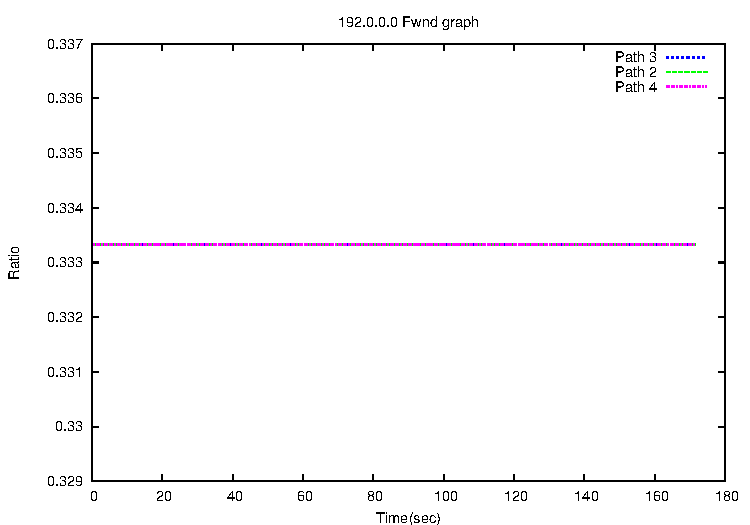
\epsfig{file=img/results/fwnd-192-0-0-0, width=4.5in}
\caption{
  Flowlet ratio $f_{i}$ for destination $E_{1}$ as set by ingress point $I_{1}$.
    \label{fig:fwnd}
}
 \end{center}
\end{figure}

The graphs bellow show the throughput of the traffic that ingress node I1 send over each link.\\

PREF

\begin{figure}[h]
 \begin{center}

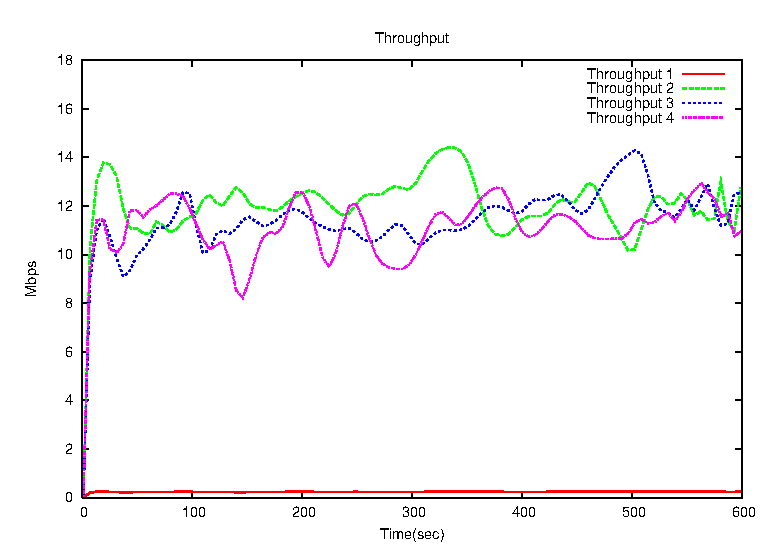
\epsfig{file=img/results/sec5-1/equalization-PREF/eleven/throuputs, width=4.5in}
\caption{
  Throughputs over each interface.
    \label{fig:equal-thro-pref}
}
\end{center}

FLARE

\end{figure}

 \begin{figure}[h!]
 \begin{center}
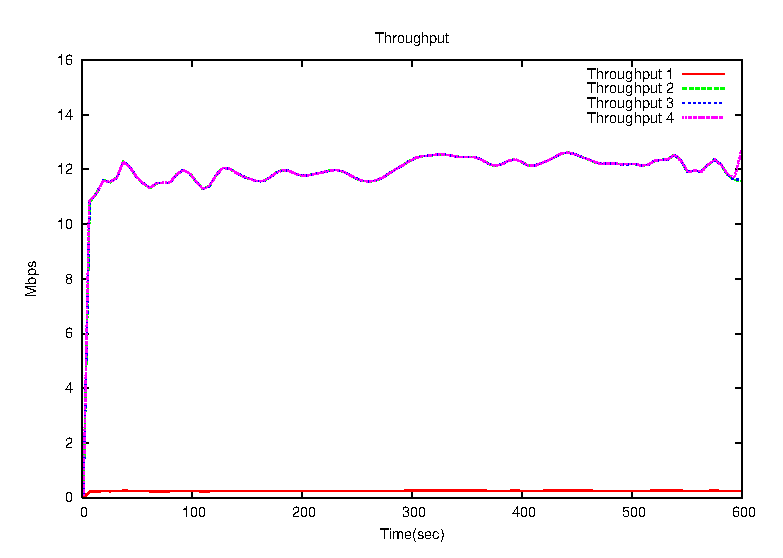
\epsfig{file=img/results/sec5-1/equalization-FLARE/eleven/throuputs, width=4.5in}
\caption{
  Throughputs over each interface.
    \label{fig:equal-thro-flare}
}
\end{center}

\end{figure}

%\begin{figure}[h]
%  \begin{center}
%    \mbox{
%      \subfigure[]{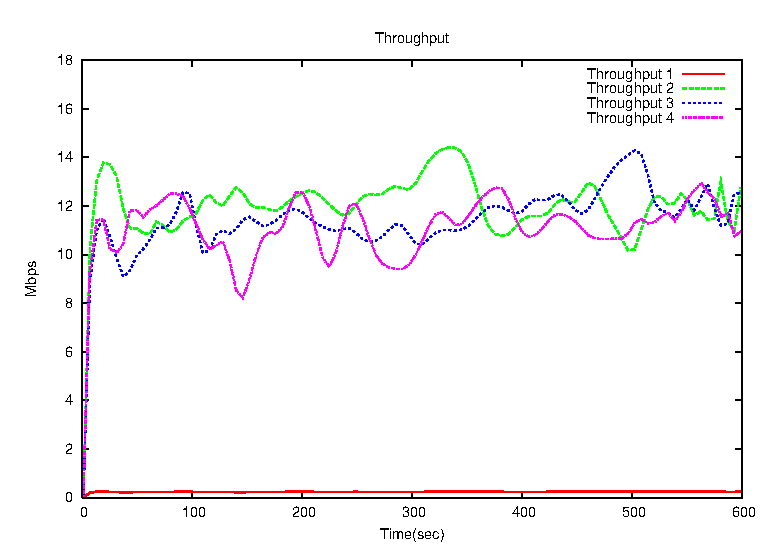
\includegraphics[width=4.0in]{img/results/sec5-1/equalization-PREF/eleven/throuputs}}\\
%      \subfigure[]{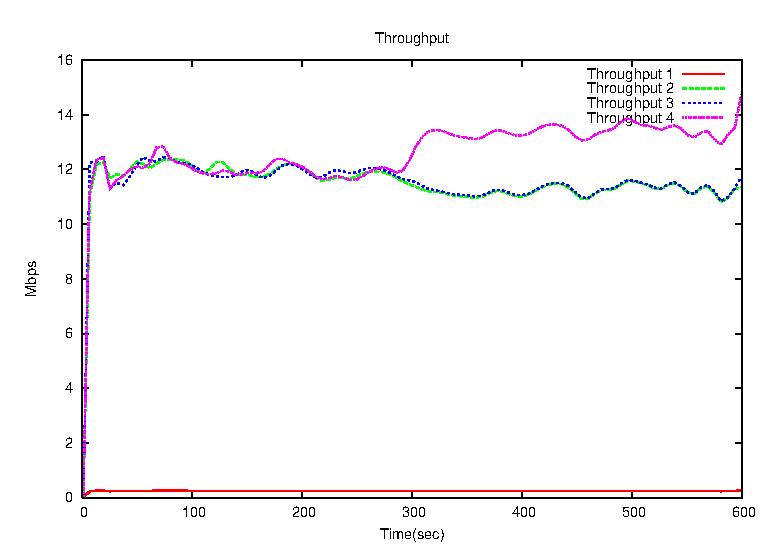
\includegraphics[width=4.0in]{file=img/results/sec5-1/equalization-FLARE/eleven/throuputs}}
%    }
%\caption{caption goes here.}
%\label{fig:parts}
%\end{center}
%\end{figure}

As expected, PREF which is equilibrium a flow based traffic splitter, doesn't match the accuracy level of FLARE in splitting the traffic, but still the difference on the throughput over each path stays limited. The graphs also show oscillation behavior of PREF. We find the same oscillation behavior in the graphs of drop rate at the bottlenecks.

PREF

\begin{figure}[h]
 \begin{center}

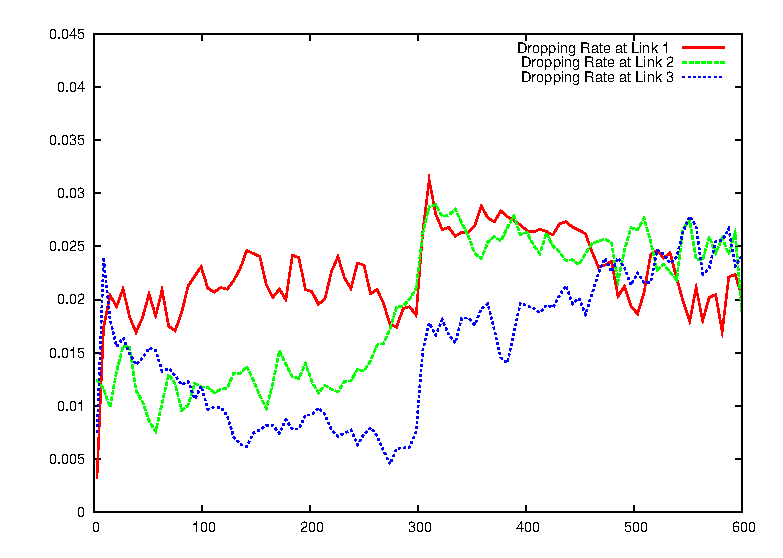
\epsfig{file=img/results/sec5-1/equalization-PREF/dropRate, width=4.5in}
\caption{
  Drop Rate at the botlenecks.
    \label{fig:equal-thro-pref}
}
\end{center}
\end{figure}

FLARE
 \begin{figure}[h!]
 \begin{center}
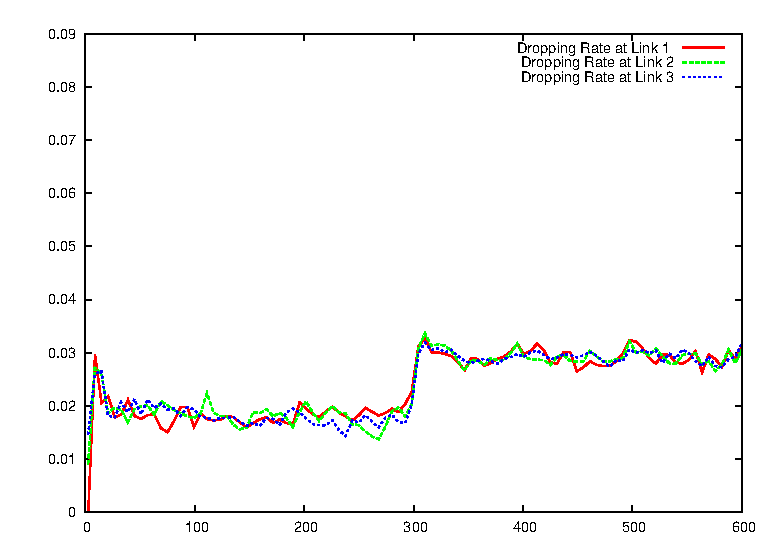
\epsfig{file=img/results/sec5-1/equalization-FLARE/dropRate, width=4.5in}
\caption{
  Drop Rate at the botlenecks.
    \label{fig:equal-thro-flare}
}
\end{center}
\end{figure}

These seconds graphs provide a hint about the reason of the fluctuation. The path assignment process of PREF makes the flowlets, which are transport aware, evolve their whole life cycle in one path and hence have a different congestion experience than the other flows. As a result, their transmission rates and the congestion they make are decorrelated. In the other hand, the network flowlets used by FLARE are a smaller order of granuilarity and makes that the transport flows get a path attributed multiple times during their flow time. As a result, the congestion level that a TCP routine experienced is a combination of the congestion in the different paths and hence the flows adapt their transmission rate to a common level of congestion and the fluctuations are less significant.

%\clearpage

\subsection{balancing by path utilization}

Now we consider the example of balancing by path utilization, a simplified version of TEXCP where ingress points don't use the core routers feedback to control their transmissions rate.

PREF

\begin{figure}[h]
 \begin{center}

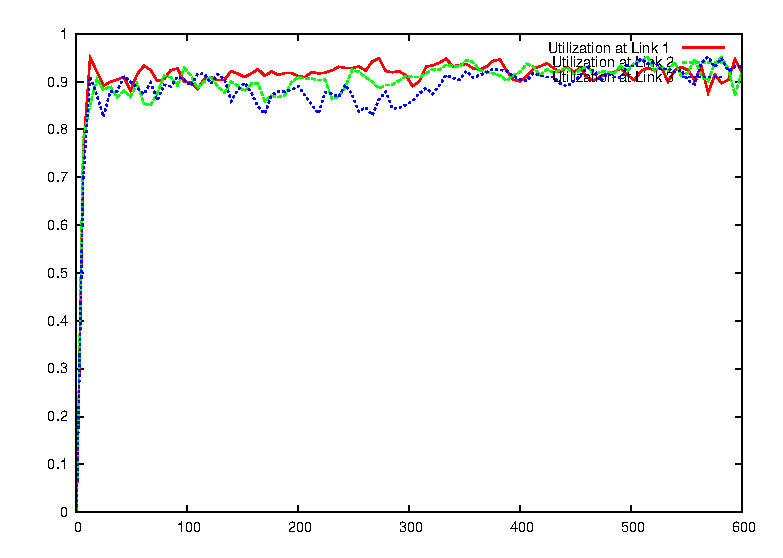
\epsfig{file=img/results/sec5-1/equalization-PREF/util, width=4.5in}
\caption{
  Path utilization measured at bottlenecks. 
    \label{fig:texcp-util-pref}
}
\end{center}
\end{figure}

FLARE
 \begin{figure}[h!]
 \begin{center}
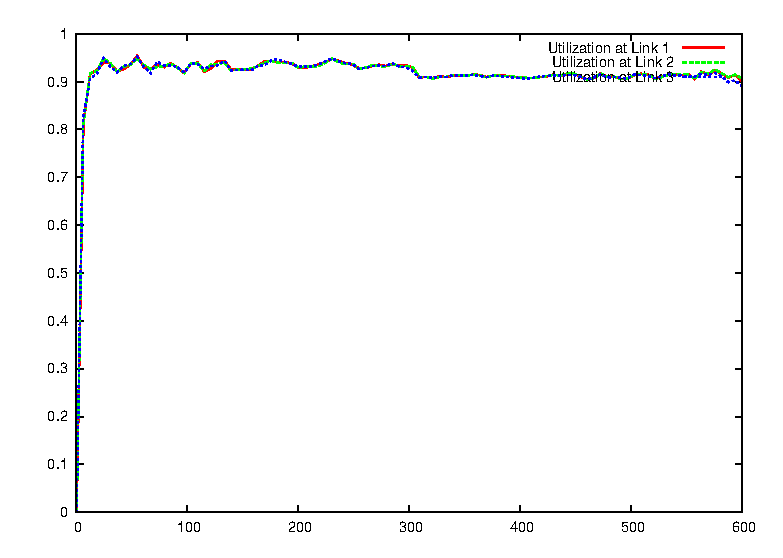
\epsfig{file=img/results/sec5-1/texcp-flare/util, width=4.5in}
\caption{
  Path utilization measured at bottlenecks. 
    \label{fig:texcp-util-flare}
}
\end{center}
\end{figure}

The previous analysis is stil valid ine the case of balamcing by path utilization. This last parameter oscillates in the case of PREF splitting, and equalization is not achieved with the same accuracy.

\paragraph{Conclusion}

Splitting traffic using PREF is required for the congestion mechanism defined by LEX. The revelation of a path congestion requires that the retransmitted packets follow the same path. Moreover, it makes congestion balancing a bit more difficult since the flows follow one path with decorelated congestion experiences. However, PREF allows path diversity schemes at end hosts and network to coexist. The performance of PREF could be enhanced further, if efficient strategies of how and when to trigger path selection were deployed at by the recievers.
 
%\section{Load balancing VS congestion balancing}
\section{Analysis of PREFLEX balancing algorithm}

In this section we are going to evaluate the performance of the algorithm for different configuration parameters. 

\subsection{Decision time interval}

The decision time interval is an external parameter for the algorithm. It determines how often the network domain updates the split. The stability of the algorithm and how long it takes to reach equilibrium is linked to the decision interval. But from another hand, this decision interval is also dependant of the period over which the loss signals are aggregated. As a result, a frequent update of the split may result in an instability of the system that will be even stressed when the aggregation time of the losses is carried out for small periods of time. In practice, we choose the decision time interval to the double of the time value for the aggregation.

The graphs bellow show the dropping rate observed at the bottleneck. 

\begin{figure}[h]
 \begin{center}

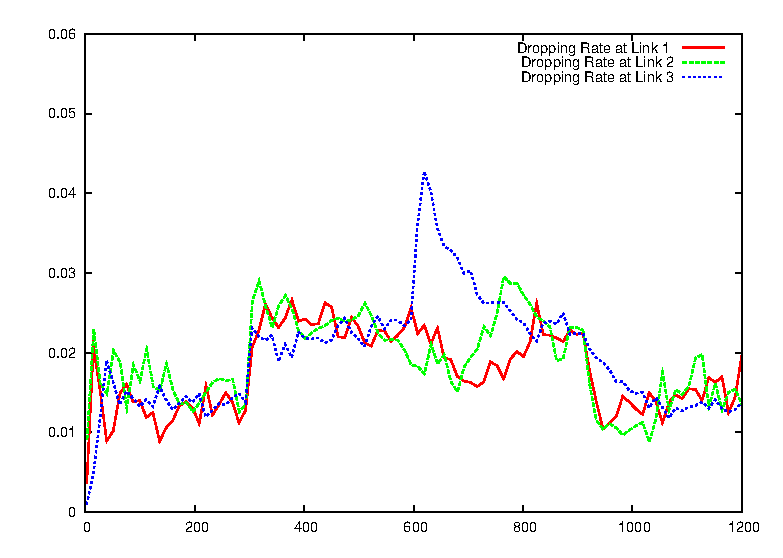
\epsfig{file=img/sec-5-2-1/eight/dropRate, width=4.5in}
\caption{
  Drop Rate at the botlenecks. 
    \label{fig:split-eight}
}
\end{center}
\end{figure}

%FLARE
 \begin{figure}[h!]
 \begin{center}
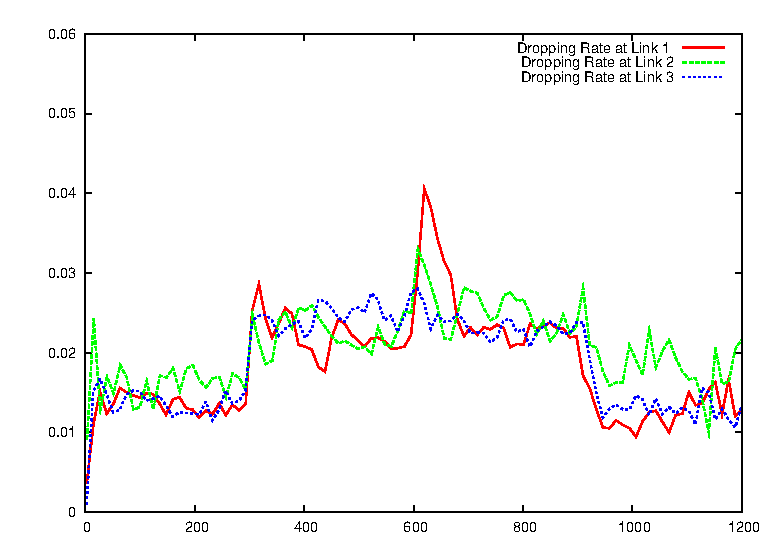
\epsfig{file=img/sec-5-2-1/four/dropRate, width=4.5in}
\caption{
  Drop Rate at the botlenecks.
    \label{fig:split-time-four}
}
\end{center}
\end{figure}

\clearpage

{\bf Update interval: 1sec}

\begin{figure}[h]
 \begin{center}

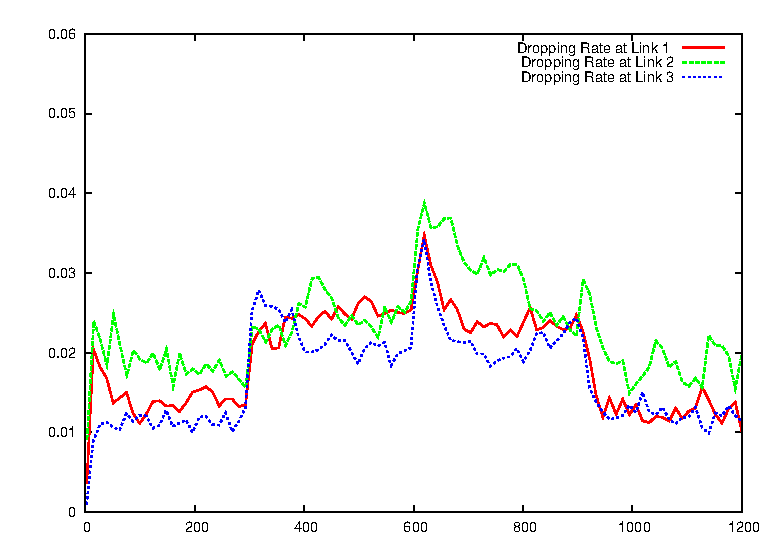
\epsfig{file=img/sec-5-2-1/one/dropRate, width=4.5in}
\caption{
  Drop Rate at the botlenecks.
    \label{fig:split-one}
}
\end{center}
\end{figure}

As expected, with a small update interval the algorithm acts more aggressively and doesn't leave enough time for the flows to reach stability. As a result the congestion level experienced in the different paths (expressed by the dropping rate at each bottleneck) is not well balanced. A larger time intervals (8 and 4 sec) allow to achieve a better balancing of the congestion over the available paths and with an enhanced stability. From the different simulations that we've carried out, an update interval between 40 to 100 RTT (approximately 100ms for the simulations here) allowed to achieve most of the time a good accuracy of the congestion balancing. An even higher value for the update interval turns the balancer too slow. This effect could be illustrated with the reaction of the system for sudden and important change in traffic demand. We could see at around the second 600, when the demand on traffic turned from a destination to another one, the balancer with an update interval of 4 sec required slightly less time to achieve equilibrium.    
 
 \clearpage

%\begin{figure}[htbp]
%\begin{center}
%\subfloat[]{
%\label{rcpstart4}
%\includegraphics[scale=0.4]{plots/lan/1.5Mb/rcp/flowstart4.eps}}
%\hspace{10mm}
%\subfloat[]{
%\label{xcprcpstart4}
%\includegraphics[scale=0.4]{plots/lan/1.5Mb/xcp0/flowstart4.eps}}
%\caption{The throughput of end-hosts and the router queue as a fourth flow starts, using \protect\subref{rcpstart4} RCP and \protect\subref{xcprcpstart4} XCP.}
%\label{rcpstart4comp}
%\end{center}
%\end{figure}

\subsection{PREFLEX balancing modes}

In this section we are going to analyse PREFLEX balancing mode: Equalization, Conservative and Loss Driven.

Reminder
$\beta_{E}$, $\beta_{C}$ and $\beta_{L}$ denotes positive factors associated consecutively with “equalization” $E$, “conservative” $C$, and “loss driven” $L$ modes.

{\bf Conservative mode} : $\beta_{E}=0$, $\beta_{C}=1$ and $\beta_{L}=0$
\\The conservative mode doesn't achieve an accurate congestion balancing over the available paths (figure \ref{fig:splitCon-loss}). But more importantly, the split as desired by the balancer in this mode is not stable(figure \ref{fig:splitCon-fwnd}). Thus, it can't be used to stabilize the performance of the balancer. A plausible explanation is limitation of the assumption that the flow fraction is equal to byte fraction, when the loss rates of paths aren't equivalent.

\begin{figure}[h!]
 \begin{center}

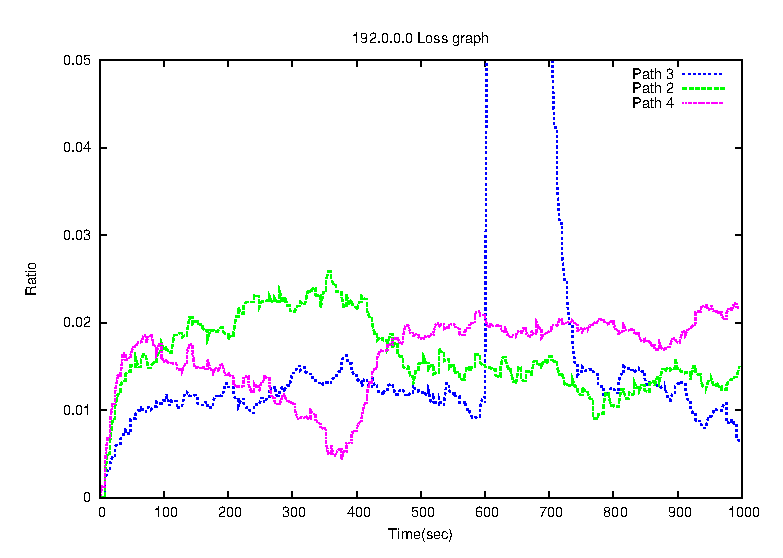
\epsfig{file=img/sec-5-2-2/Alt-split-0-100-0/loss-192-0-0-0, width=4.5in}
\caption{
   Loss ratio $\rho_{i}$ for destination E1 as seen by balancer P in consrvative mode.

    \label{fig:splitCon-loss}
}
\end{center}
\end{figure}

\clearpage
\begin{figure}[h!]
 \begin{center}

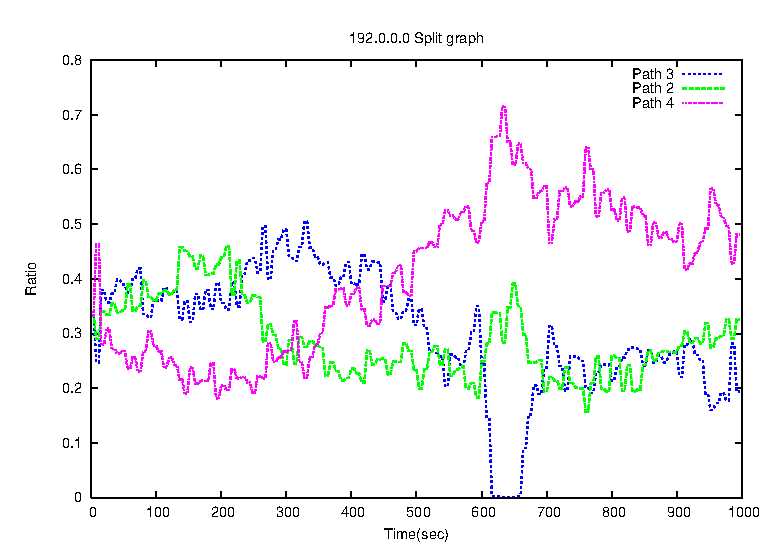
\epsfig{file=img/sec-5-2-2/Alt-split-0-100-0/fwnd-192-0-0-0, width=4.5in}
\caption{
   The desired split that balancer P set for destination E1 in conservative mode.

    \label{fig:splitCon-fwnd}
}
\end{center}
\end{figure}


{\bf Equalization} : $\beta_{E}=1$, $\beta_{C}=0$ and $\beta_{L}=0$
\\As depicted by figure \ref{fig:splitEqual-loss}, an equal distribution of flows over the paths doesn't achieve an equal balancing of loss. Moreover, its performance depends on the traffic nature in the network. Path 3 underutilized illustrates the suboptimal nature of equal balancing. Also the difference of congestion levels in the other two paths is directly linked to changes in traffic demand. During the change on traffic demand between time 200sec and 600sec, the difference between the congestion levels significantly increased.

However, the real contribution of the "equal" mode is to ensure that a minimum number of flows are sent over each path. In fact, as we are going to see next, the accuracy of the loss estimation made by the loss balancer depends on the number of flows sent over the path. 

\clearpage
\begin{figure}[h]
 \begin{center}

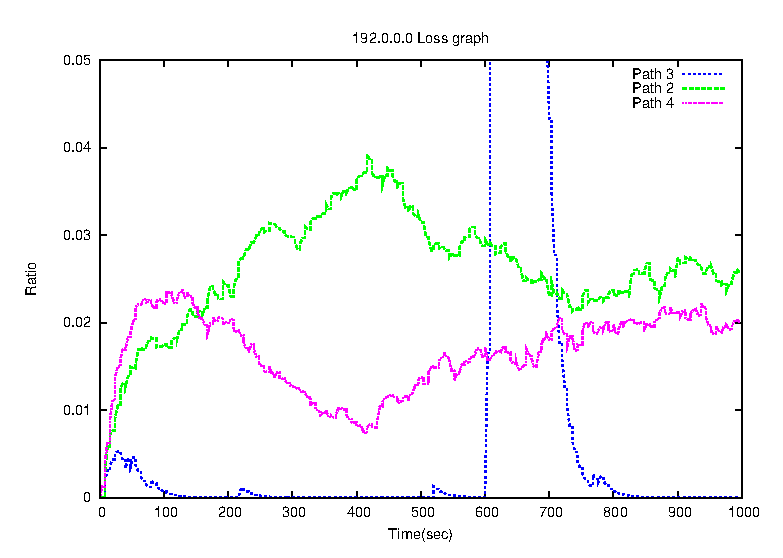
\epsfig{file=img/sec-5-2-2/Alt-split-0-0-100/loss-192-0-0-0, width=4.5in}
\caption{
   Loss ratio $\rho_{i}$ for destination E1 as seen by balancer P in equalisation mode.

    \label{fig:splitEqual-loss}
}
\end{center}
\end{figure}


{\bf Unbounded loss driven mode} : $\beta_{E}=0$, $\beta_{C}=0$ and $\beta_{L}=1$
\\Figures \ref{fig:splitpureLoss-fwnd1} and \ref{fig:splitpureLoss-fwnd1} show that the balancer allocate different splits for destination E1 and E2 even when the system is symmetric for the two destinations. This is explained by the fact that balancing for the two destination is carried separately which is natural since the flows for the two destinations. This is natural since the paths for the two destinations are different even if they share the same bottleneck in our topology. But there is no one optimal split, and the balancer succeeds though during the first 200 sec in balance the congestion equally for both destination (see \ref{fig:splitpureLoss-loss1} and \ref{fig:splitpureLoss-loss2}). But by keeping to send less E2 flows on the path, the accuracy of the loss estimation become low and different from E1 flows. In particular, it is over estimated what accelerate more the drop. As a result the equalization mode is used to make sure that there are enough flows on every path for an accurate estimation of the loss.

\begin{figure}[h]
 \begin{center}

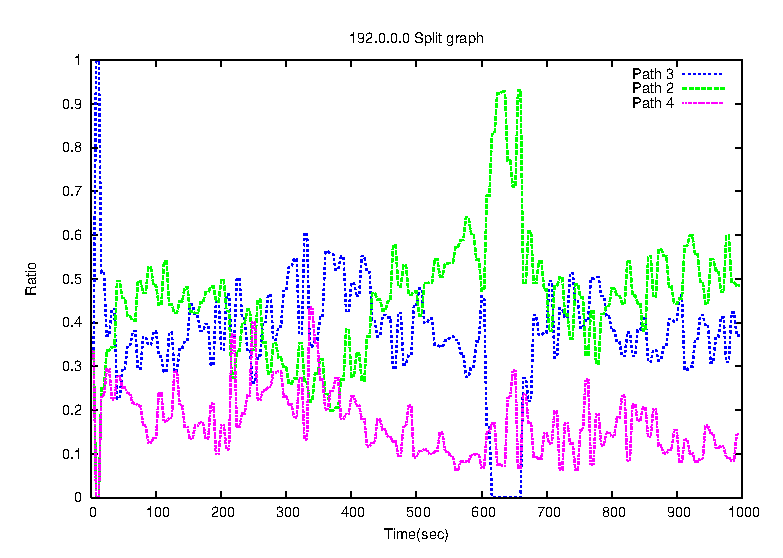
\epsfig{file=img/sec-5-2-2/Alt-split-100-0-0/fwnd-192-0-0-0, width=4.5in}
\caption{
   The desired split that balancer P set for destination E1 in unbounded loss driven mode.

    \label{fig:splitpureLoss-fwnd1}
}
\end{center}
\end{figure}

\begin{figure}[h]
 \begin{center}

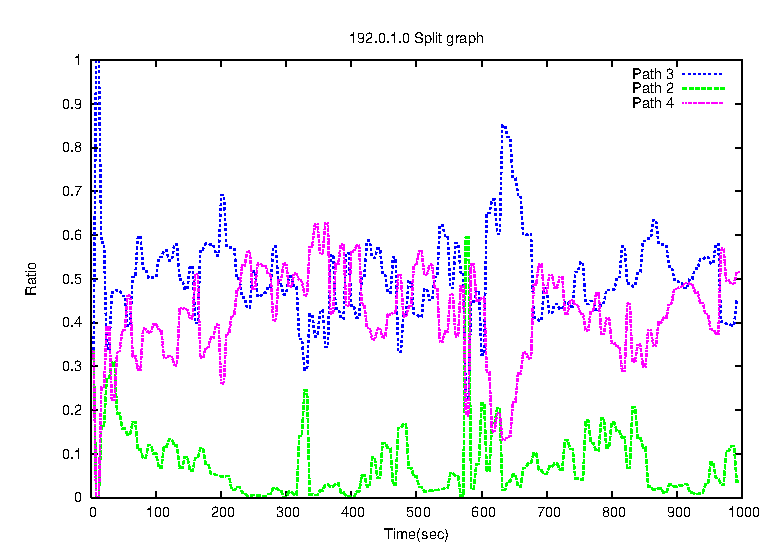
\epsfig{file=img/sec-5-2-2/Alt-split-100-0-0/fwnd-192-0-1-0, width=4.5in}
\caption{
   The desired split that balancer P set for destination E2 in unbounded loss driven mode.

    \label{fig:splitpureLoss-fwnd2}
}
\end{center}
\end{figure}


\begin{figure}[h]
 \begin{center}

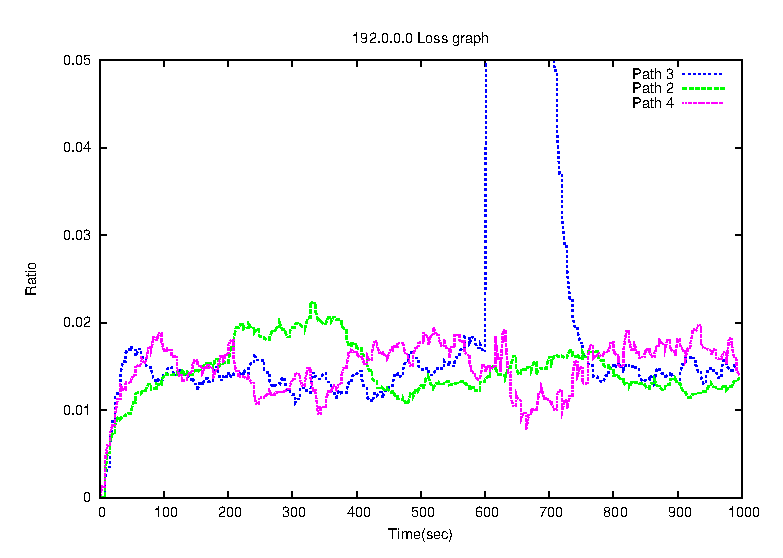
\epsfig{file=img/sec-5-2-2/Alt-split-100-0-0/loss-192-0-0-0, width=4.5in}
\caption{
   Loss ratio $\rho_{i}$ for destination E1 as seen by balancer P in unbounded loss driven mode.

    \label{fig:splitpureLoss-loss1}
}
\end{center}
\end{figure}

\begin{figure}[h]
 \begin{center}

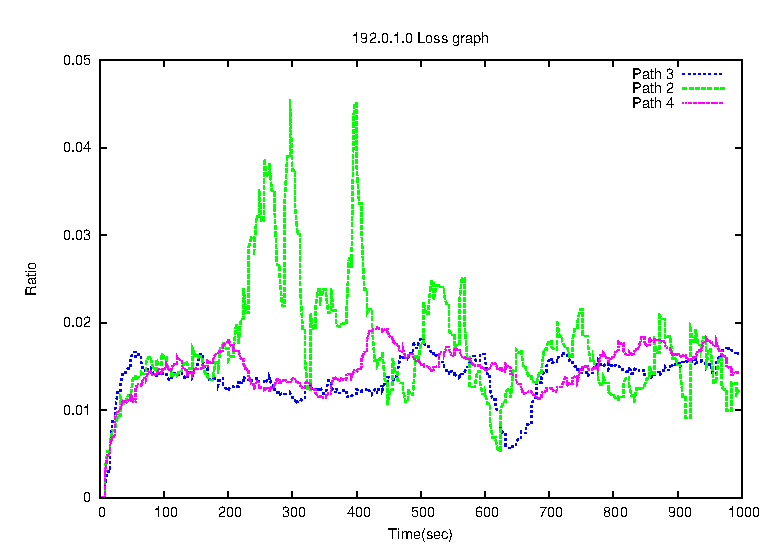
\epsfig{file=img/sec-5-2-2/Alt-split-100-0-0/loss-192-0-1-0, width=4.5in}
\caption{
   Loss ratio $\rho_{i}$ for destination E2 as seen by balancer P in unbounded loss driven mode.

    \label{fig:splitpureLoss-loss2}
}
\end{center}
\end{figure}

\clearpage

{\bf Bounded loss driven mode} : $\beta_{E}=0.9$, $\beta_{C}=0$ and $\beta_{L}=0.1$
\\By allocating a share of the traffic to be equally distributed we guarantee that a minimum number of flows is sent over each path to continue probing the path in question and accurately estimate its level of congestion. The effect of this boundary is clearly shown in the loss distribution compared to the previous mode \ref{fig:splitlossD-loss1} and \ref{fig:splitlossD-loss2}. Though, the  booked share for equalization should be too high to block the loss equalization process. 

In another hand, \ref{fig:splitlossD-fwnd1} and \ref{fig:splitlossD-fwnd1} {\bf Something about failure}


\begin{figure}[h]
 \begin{center}

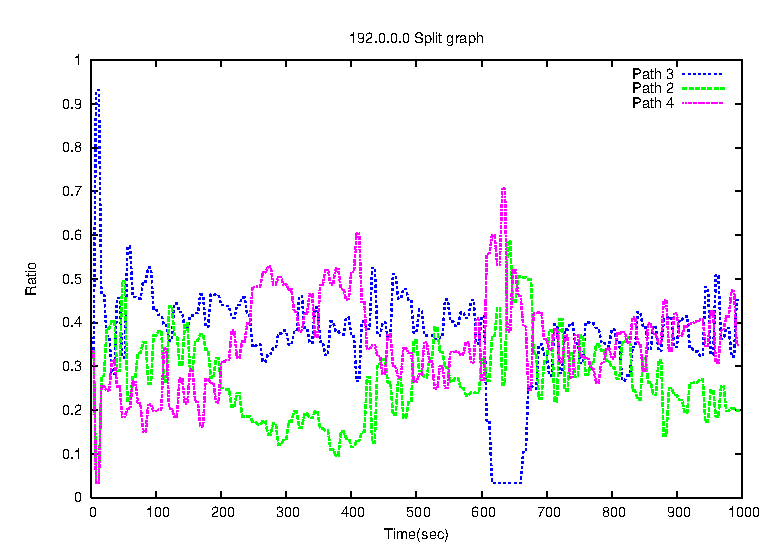
\epsfig{file=img/sec-5-2-2/Alt-split-90-0-10/fwnd-192-0-0-0, width=4.5in}
\caption{
   The desired split that balancer P set for destination E1 in "pure" loss driven mode.

    \label{fig:splitlossD-fwnd1}
}
\end{center}
\end{figure}

\begin{figure}[h]
 \begin{center}

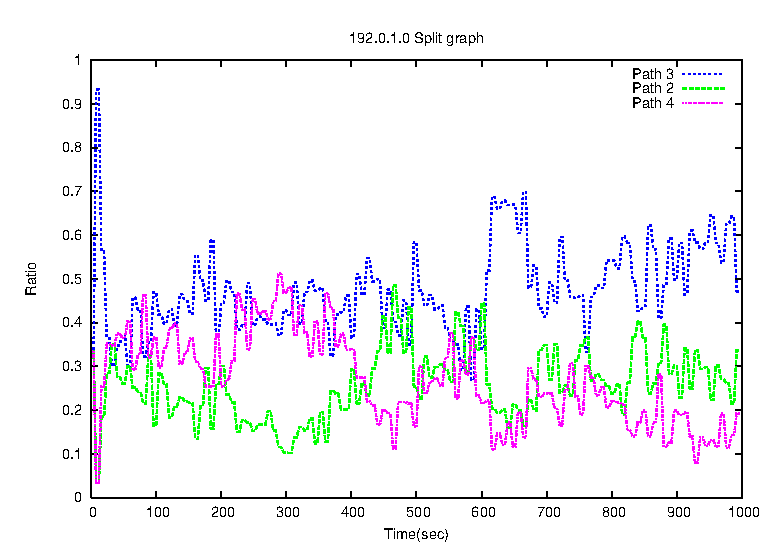
\epsfig{file=img/sec-5-2-2/Alt-split-90-0-10/fwnd-192-0-1-0, width=4.5in}
\caption{
   The desired split that balancer P set for destination E2 in "pure" loss driven mode.

    \label{fig:splitlossD-fwnd2}
}
\end{center}
\end{figure}


\begin{figure}[h]
 \begin{center}

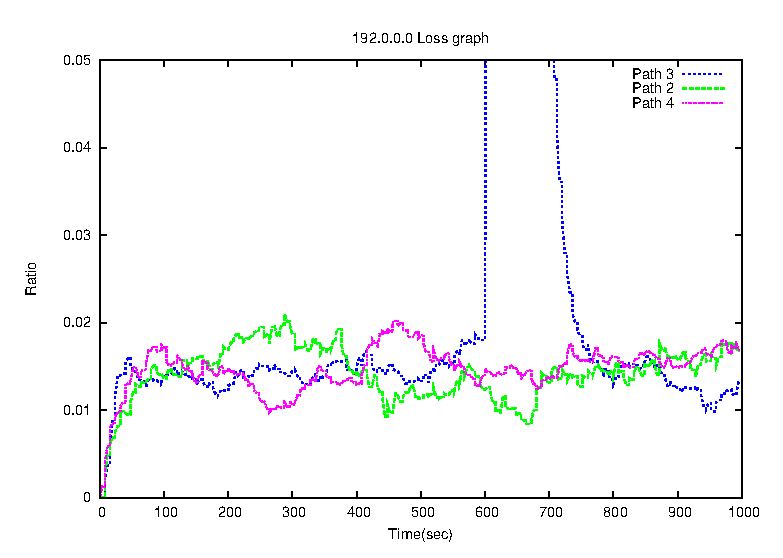
\epsfig{file=img/sec-5-2-2/Alt-split-90-0-10/loss-192-0-0-0, width=4.5in}
\caption{
   Loss ratio $\rho_{i}$ for destination E1 as seen by balancer P in "pure" loss driven mode.

    \label{fig:splitlossD-loss1}
}
\end{center}
\end{figure}

\begin{figure}[h]
 \begin{center}

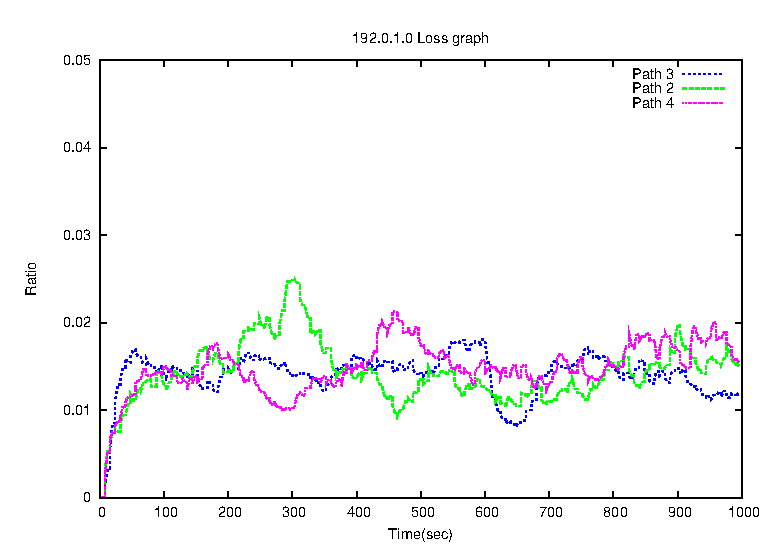
\epsfig{file=img/sec-5-2-2/Alt-split-90-0-10/loss-192-0-1-0, width=4.5in}
\caption{
   Loss ratio $\rho_{i}$ for destination E2 as seen by balancer P in "pure" loss driven mode.

    \label{fig:splitlossD-loss2}
}
\end{center}
\end{figure}

\clearpage

\section{Comparison between PREFLEX and TEXCP}

{\bf Balancing by path utilization}
\\In this section we consider a simplified version of TEXCP (the same as in 5.1.1) that balances path utilization but doesn't activate TEXCP congestion management measures and only balance the path utilization. As expected (figure \ref{fig:st-util}), the modified version do very well in equalizing the path utilization, reacting very quickly to changes in network traffic state while keeping a stable behavior. 

However, by looking at the drop rate in bottlenecks (figure \ref{fig:st-drop}) we observe that it is not equal on the different links. This observation, have a meaningful explanation behind. The high frop rate on the likn is compensated by a higher load (received bytes over the capacity) so the utilization is equal on the three links. This means that using only this measure for balancing the load we risk to drive the network to a suboptimal state. The other observation is about the loss level that ingress routers see using LEX codepoint (figure \ref{fig:st-loss1}). All the three interfaces, which correspond to the links, have the same level. This is an expected results since TEXP use FLARE which doesn't guarantee that retransmissions follow the same path as the original packet. This have another result is that within dew RTTs, TCP routines using different paths experience the congestion of each of them and hence they adapt their transmission rate to a combination of loss rate in each path that could be estimated as:

\begin{equation}
\rho = \sum_{i} x_{i}\cdot \rho_{i} 
\end{equation}

where, $\rho_{i}$ and $x_{i}$ are respectively the loss rate and the probability to take path i. But we should keep in mind that such high levels of path utilization aren't frequent in intra-domain TE, since not all the flows are elastic as it is the case in our scenario. For such cases, TEXCP defines a feedback mechanism to control congestion.

\begin{figure}[h]
 \begin{center}

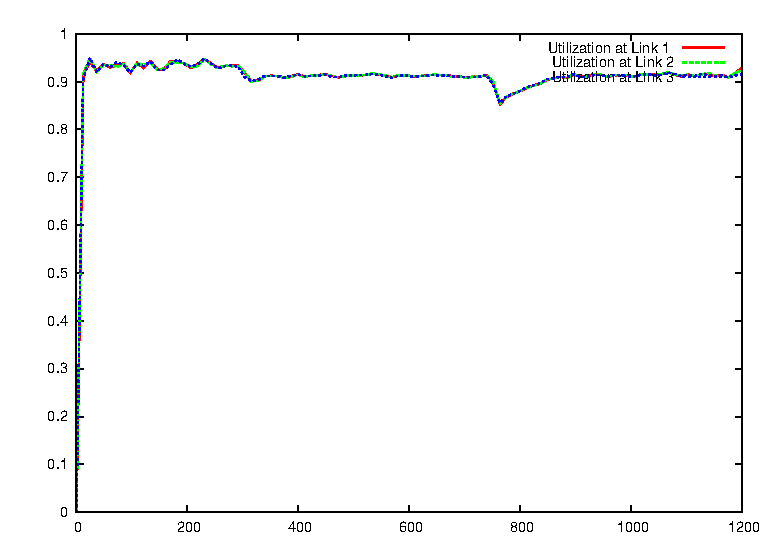
\epsfig{file=img/sec-5-2-3/no-traffic-shaper/util, width=4.5in}
\caption{
   The link utilization measured at the bollenecks in simplified TEXCP.

    \label{fig:st-util}
}
\end{center}
\end{figure}

\begin{figure}[h]
 \begin{center}

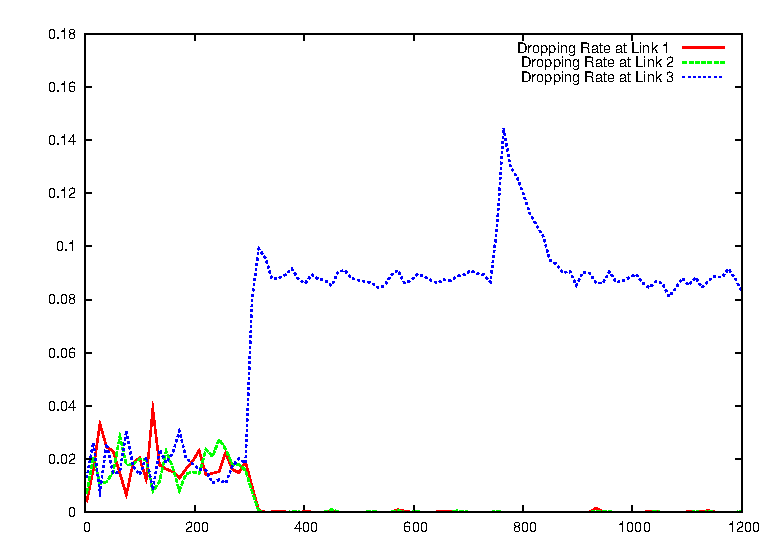
\epsfig{file=img/sec-5-2-3/no-traffic-shaper/dropRate, width=4.5in}
\caption{
   The drop rate measured at the bollenecks in simplified TEXCP.

    \label{fig:st-drop}
}
\end{center}
\end{figure}

\begin{figure}[h]
 \begin{center}

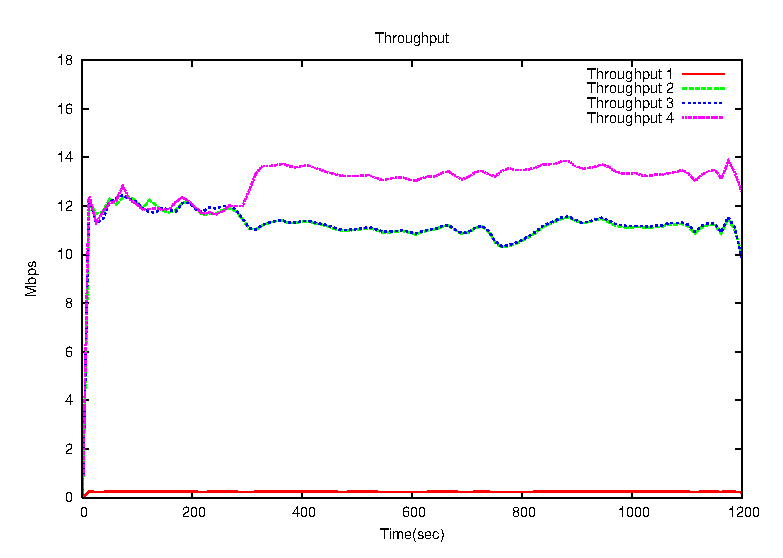
\epsfig{file=img/sec-5-2-3/no-traffic-shaper/10/throuputs, width=4.5in}
\caption{
   The throughput measured at ingress router I1 interfaces in simplified TEXCP.

    \label{fig:st-fwnd}
}
\end{center}
\end{figure}

\begin{figure}[h]
 \begin{center}

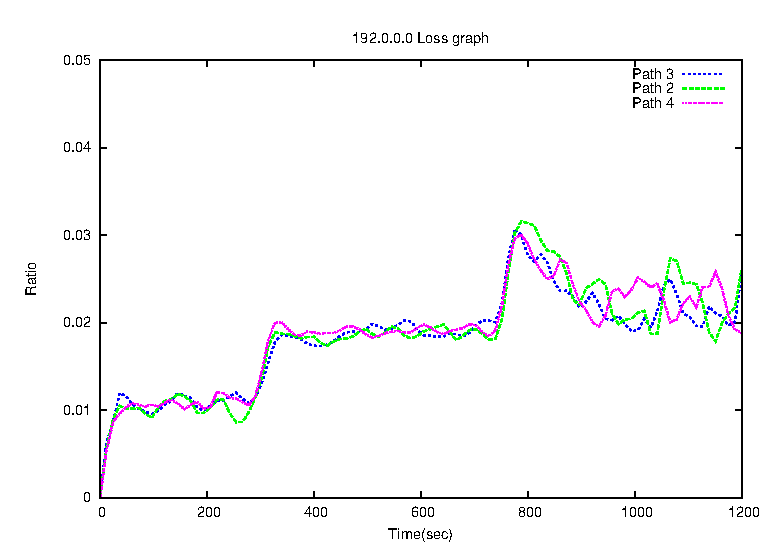
\epsfig{file=img/sec-5-2-3/no-traffic-shaper/10/loss-192-0-0-0, width=4.5in}
\caption{
   Loss ratio $\rho_{i}$ for destination E1 as seen by balancer ingress router I1 in simplified TEXCP.

    \label{fig:st-loss1}
}
\end{center}
\end{figure}
\clearpage 

{\bf TEXCP}

\\In this section TEXCP was fully implemented. A traffic shaper is associated with each Ingress/Egress route and control the transmission rate over the different paths. The path utilization is still equalized for the three bottlenecks (figure \ref{fig:t-util}), but most importantly the difference in drop rate ???? at each link disappeard (\ref{fig:t-drop}). The path utilization has slightly increase, which is correlated with the decrease in the drop rate at the bottleneck since TCP routing under low loss rate have a stable transmission rate and doesn't fluctuate a lot. By limiting the transmission rate, the effect of the traffic shaper is to move congestion and more precisely the dropping from the core network to the edge. 

The introduction of traffic shapers changes the loss rate. Indeed, traffic shaper allocates a buffer for each destination instead of the common buffer at the bottlneck. In our topology each link pass through the traffic of four IE pairs. Using traffic shapers means that four queues will be added. The number of added queue and their size are new parameters to influence the level of congestion. For instance the ratio buffer size over the transmission rate could decrease significantly the global loss rate if set to a high value, and the inverse is true. The mathematical formalization of this problem is quite difficult.

But the drawback of the use traffic shapping and transmission rate control, is to equally distributed bandwidth over pairs but not according to the size of traffic travelling between them. In general this results in a bandwidth waste since some of the users won't be able to use all their share. But since we are using elastic flow the bandwidth is fully used, yet the level of loss is different from a destination to another (figure \ref{fig:t-loss1} and \ref{fig:t-loss2}). Starting from the moment when the bottlenecks feel congested, the transmission rate of each pair and path is decreased. The decrease mechanism is multiplicative, so if the transmission rates were defined equally at the beginning they will reach the same equilibrium. This is fine while they have equal number of flows but once this distribution change the different flows will keep having equal rates. This means that the level of congestion experience for one destination is different from another even if they share the same bottleneck. Hence the use of traffic shappers introduce unfairness.

\begin{figure}[h]
 \begin{center}

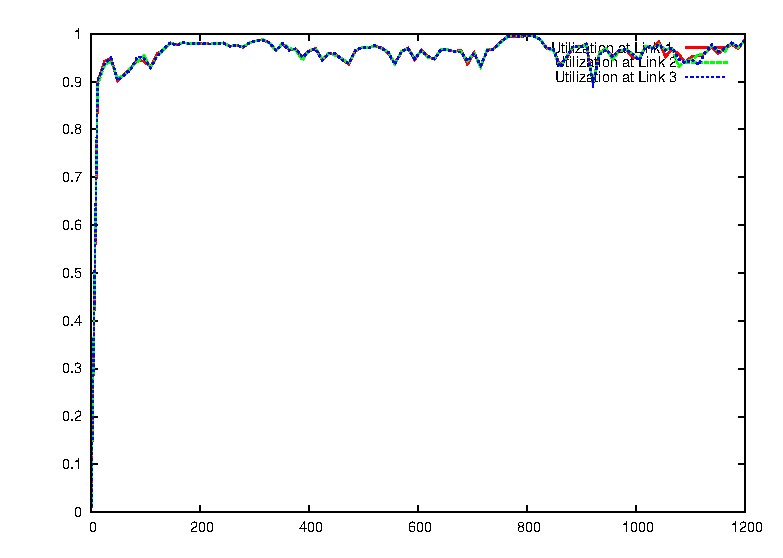
\epsfig{file=img/sec-5-2-3/trafficShaper/util, width=4.5in}
\caption{
   The link utilization measured at the bollenecks in TEXCP.

    \label{fig:t-util}
}
\end{center}
\end{figure}

\begin{figure}[h]
 \begin{center}

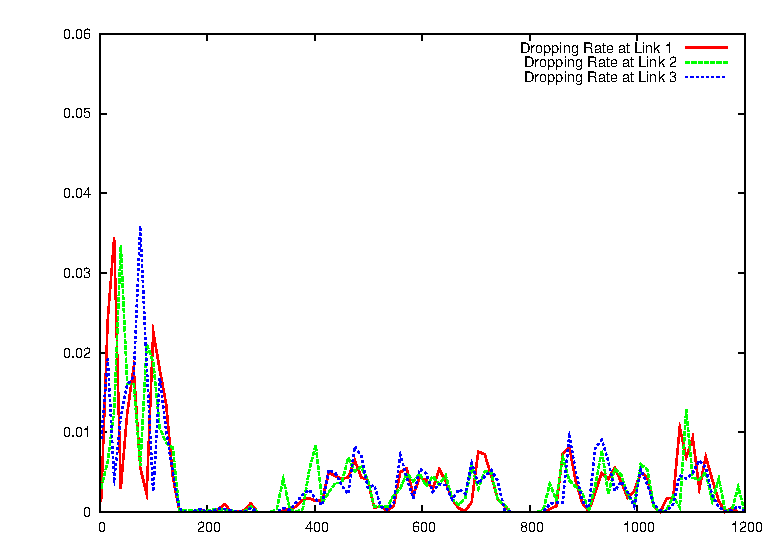
\epsfig{file=img/sec-5-2-3/trafficShaper/dropRate, width=4.5in}
\caption{
   The drop rate measured at the bollenecks in TEXCP.

    \label{fig:t-drop}
}
\end{center}
\end{figure}

\begin{figure}[h]
 \begin{center}

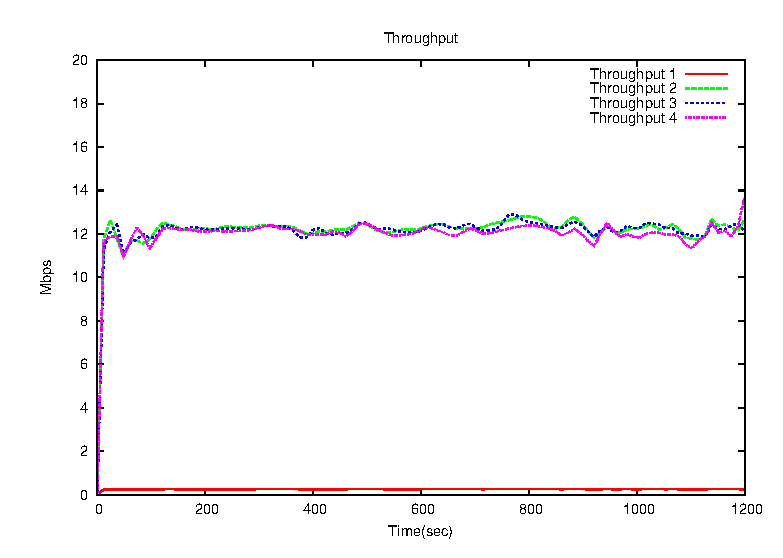
\epsfig{file=img/sec-5-2-3/trafficShaper/10/throuputs, width=4.5in}
\caption{
   The throughput measured at ingress router I1 interfaces in TEXCP.

    \label{fig:t-fwnd}
}
\end{center}
\end{figure}

\begin{figure}[h]
 \begin{center}

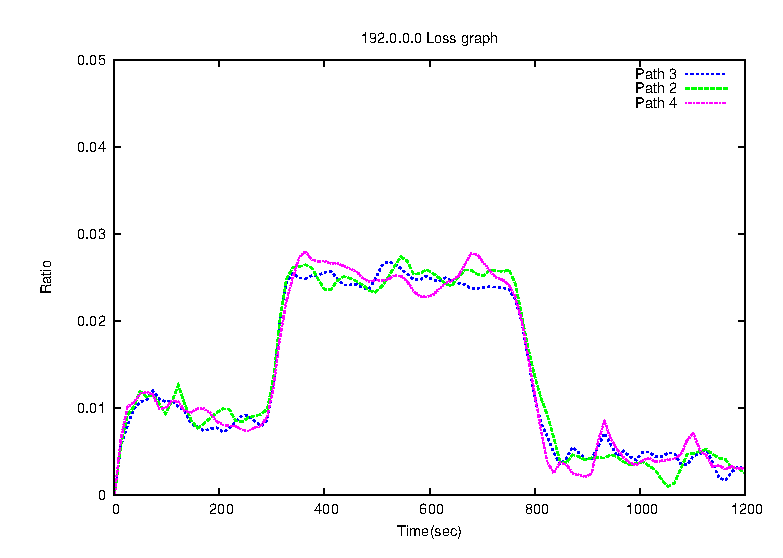
\epsfig{file=img/sec-5-2-3/trafficShaper/10/loss-192-0-0-0, width=4.5in}
\caption{
   Loss ratio $\rho_{i}$ for destination E1 as seen by balancer ingress router I1 in TEXCP.

    \label{fig:t-loss1}
}
\end{center}
\end{figure}

\begin{figure}[h]
 \begin{center}

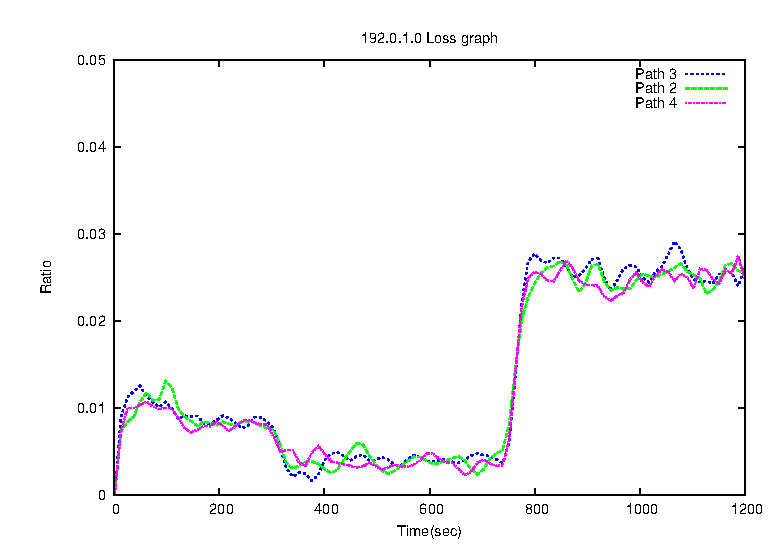
\epsfig{file=img/sec-5-2-3/trafficShaper/10/loss-192-0-1-0, width=4.5in}
\caption{
   Loss ratio $\rho_{i}$ for destination E2 as seen by balancer ingress router I1 in TEXCP.

    \label{fig:t-loss2}
}
\end{center}
\end{figure}

\clearpage 

{\bf PREFLEX}
\\ In this section a comparison is carried out with congestion balancing in PREFLEX. The congestion parameters of the balancing algorithm were set to : $\beta_{E}=0.9$, $\beta_{C}=0$ and $\beta_{L}=0.1$.

PREFLEX performance in balancing congestion is similar to the one obtained in the previous section for the same configuration (Analysis of PREFLEX balancing algorithm 5.2.2). 


\begin{figure}[h]
 \begin{center}

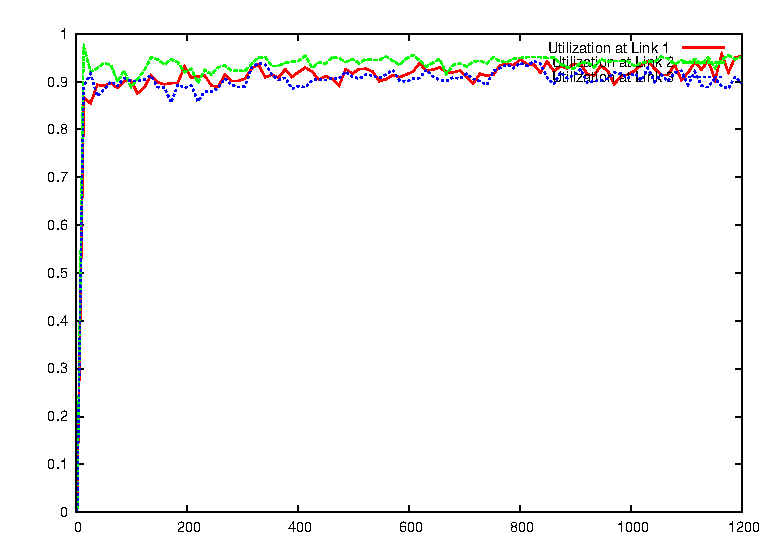
\epsfig{file=img/sec-5-2-3/split-90-0-10/util, width=4.5in}
\caption{
   The link utilization measured at the bollenecks in TEXCP.

    \label{fig:p-util}
}
\end{center}
\end{figure}

\begin{figure}[h]
 \begin{center}

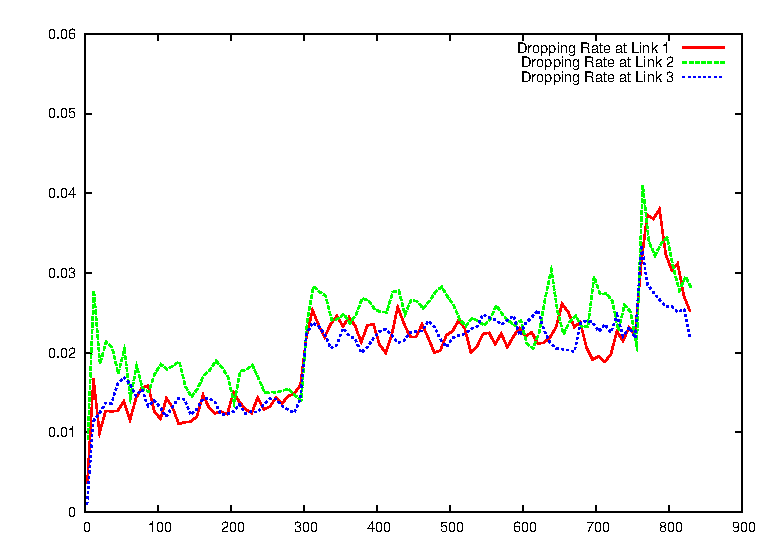
\epsfig{file=img/sec-5-2-3/split-90-0-10/dropRate, width=4.5in}
\caption{
   The drop rate measured at the bollenecks in TEXCP.

    \label{fig:p-drop}
}
\end{center}
\end{figure}

\begin{figure}[h]
 \begin{center}

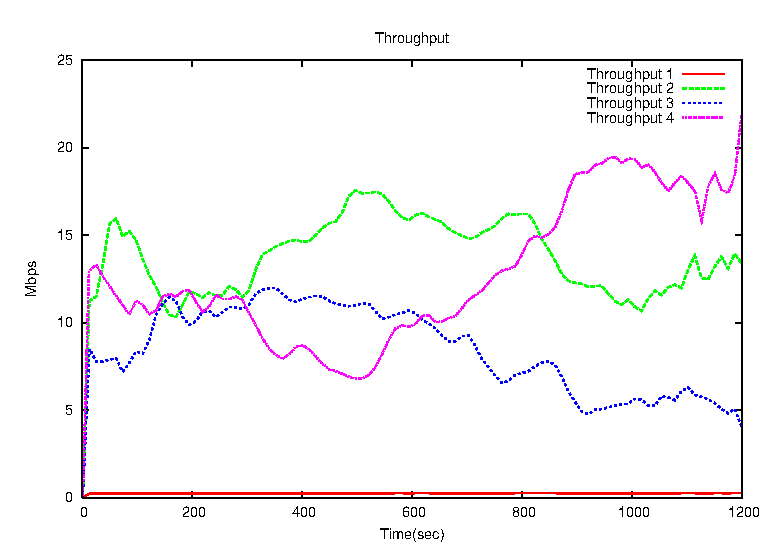
\epsfig{file=img/sec-5-2-3/split-90-0-10/10/throuputs, width=4.5in}
\caption{
   The throughput measured at ingress router I1 interfaces in TEXCP.

    \label{fig:p-fwnd}
}
\end{center}
\end{figure}

\begin{figure}[h]
 \begin{center}

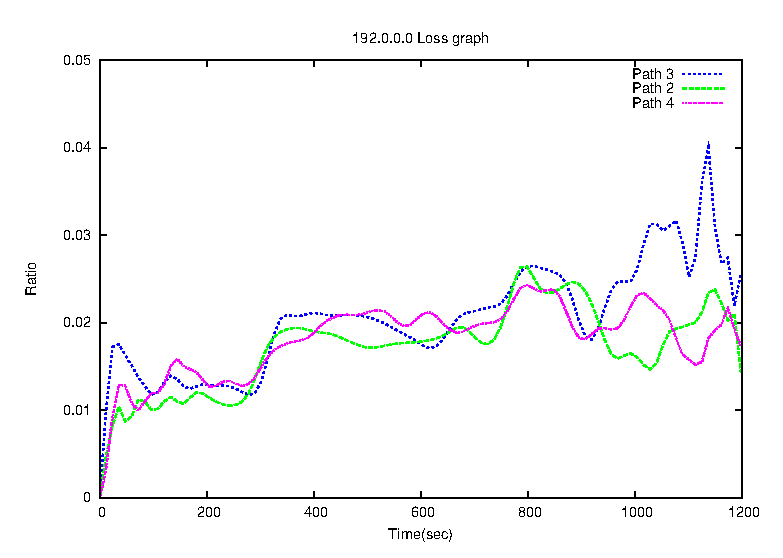
\epsfig{file=img/sec-5-2-3/split-90-0-10/10/loss-192-0-0-0, width=4.5in}
\caption{
   Loss ratio $\rho_{i}$ for destination E1 as seen by balancer ingress router I1 in TEXCP.

    \label{fig:p-loss1}
}
\end{center}
\end{figure}

\begin{figure}[h]
 \begin{center}

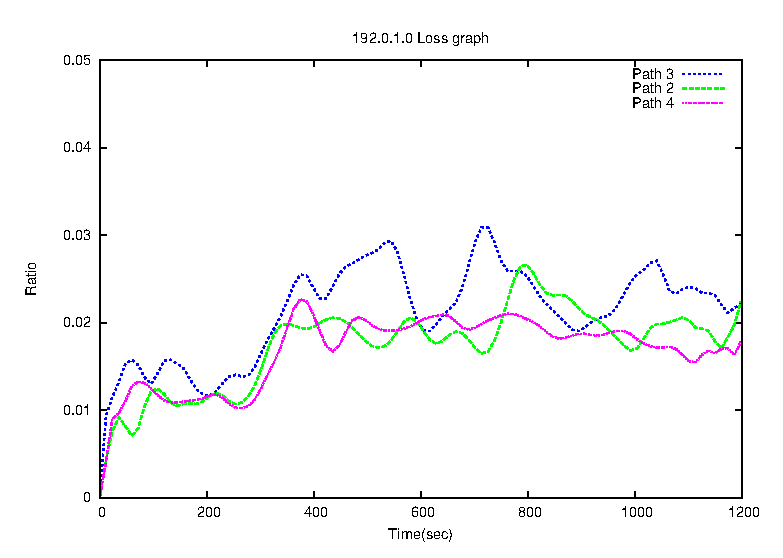
\epsfig{file=img/sec-5-2-3/split-90-0-10/10/loss-192-0-1-0, width=4.5in}
\caption{
   Loss ratio $\rho_{i}$ for destination E2 as seen by balancer ingress router I1 in PREFLEX.

    \label{fig:p-loss2}
}
\end{center}
\end{figure}


\chapter{Conclusions and future work}
\label{chap:conclusion}



\chapter{Conclusions and future work}
\label{chap:conclusion}
\section{Conclusions}

In this dissertation, the utilisation of congestion exposure for path diversity was investigatd. This concept consists on making end hosts reveal to the network the level of congestion they are experiencing. Information traditionally confined in the transport layer, will enable the network with new capabilities. Re-ECN protocol illustrated the concept and provided  to the network an effective measurement about the congestion that each customer is causing. ISPs needed this measurement to propose fair charging and police heavy users. PREFLEX uses a simple form of congestion exposure to pool path diversity. LEX the congestion exposure protocol, makes end host to tag retransmitted packet so the network could estimate the congestion level on the path that they are using. This way stub domains could allocate traffic to paths according to the level of congestion. Balancing based on congestion presents many advantages compared to the classical load balancing. 

First, by using congestion instead of resource utilization we target directly the optimization of quality of service perceived by customers. As we've seen during our analysis (section 5.3) the use of link utilization might give an illusive idea about the real state of the link.  To mitigate this problem, TEXCP is enabled with a feedback mechanism that allow congested routers to limit the transmission rate of  ingress routers. The drawback of such means is that bandwidth could be wasted and customers are not treated fairly.

Secondly, the congestion level as revealed by LEX corresponds to an end-to-end measurement contrarily to resource utilization used in TEXCP. Thus, PREFLEX architecture is not limited to intra-domain traffic engineering. Multihoming is a built-in application for the architecture.

Another feature of PREFLEX consists on the presence of cooperation between end hosts and network on multiple levels. It illustrates the fact that both parties are drawing benefits from path diversity. Thus, Path Re-Feedback, the second component of the architecture makes end hosts aware of network path preference. This information needed so the packet marked as retransmitted take the same path as the original packet. But also provides the end hosts with additional freedom regarding path diversity. It could divide the communication to potentially multiple, parallel or successive flowlets, to draw more benefits from the scheme. End hosts using optimized strategy here will draw more benefits from the architecture. Indeed the weak points of PREFLEX balancing that were observed in the simulations were mostly due to the fact that transport flows were divided on only one flowlet. Though, it is an important point to investigate for the future of the architecture.
 
\section{summary of contributions}
The work carried out during this dissertation involves participation in the definition of PREFLEX balancing algorithm. This algorithm proposes different  mode corresponding to the difference approaches for traffic balancing. The performance of these modes was analysed. Then, the performance of PREFLEX was compared to the one obtained with TEXCP. 
The analysis and simulations was conducted using a framework on ns3. The implementation was built over an existing tool. Contributions to the framework were mostly related to TEXCP. While routing agents and the queues for  core routers are only used for TEXCP, the other modules were developed in a flexible way that permit re-usability. This include the new ns3 NetDevice with traffic shaping capability and the module for packets classification needed for FLARE traffic splitting and the Traffic Shaper.  The implemented modules are functional and allow to run simulation in different configurations and topologies. 
\section{Future Work}


%\addcontentsline{toc}{chapter}{section}{Appendices}
\addcontentsline{toc}{chapter}{section}
\chapter{Appendices}
%\appendix
%\input{appendix}

\addcontentsline{toc}{chapter}{Bibliography}

\bibliography{PhD}
\begin{thebibliography}{9}
\bibitem[Araujo09]{arau1}J.Araujo, M. Rio, G. Pavlou. \emph{A Mutualistic Resource Pooling Architecture}.   2010.
\bibitem[RFC 3272]{RFC3272}D. Awduche, A. Chiu, A. Elwalid, I. Widjaja, X. Xiao. \emph{Overview and Principles of Internet Traffic Engineering}. RFC 3272, IETF, May 2002. (pp 4, 14, )
\bibitem[Awduche02]{awd1}D. Awduche, A. Chiu, A. Elwalid, I. Widjaja, X. Xiao. \emph{Overview and Principles of Internet Traffic Engineering}. May 2002.

\bibitem[Kandula05]{kan1}S. Kandula, D. Katabi, B .Davie, A. Charny. \emph{Walking the Tightrope: Responsive Yet Stable Traffic Engineering}. August 2005. 

\bibitem[Gojmerac03]{goj1}I. Gojmerac, T. Ziegler, F. Ricciato, P. Reichl. \emph{Adaptive Multipath Routing for Dynamic Traffic Engineering}. 2003.
\bibitem[Toguyni09]{tog09}A. Toguyni, O. Korbaa. \emph{DiffServ Aware MPLS Traffic
Engineering for ISP Networks: State of the Art and New Trends}. January 2009.
\bibitem[Sinha04]{sin1}S. Sinha, S. Kandula, D. Katabi. \emph{Harnessing TCPs Burstiness with Flowlet Switching}. 2004. 
\bibitem[Elwalid01]{elwal1}A. Elwalid, C. Jin, S. Low, I. Widjaja. \emph{MATE: MPLS Adaptive Traffic Engineering}. IETF, 2001. 
\bibitem[Xiao00]{xia1}X Xiao, A. Hannan, B. Bailey, L. M. Ni. \emph{Traffic Engineering with MPLS in the Internet}. IETF, 2000. 
\bibitem[Raiciu09]{rai1}C. Raiciu, D. Wischik, M. Handley. \emph{Practical Congestion Control for Multipath Transport Protocols}. 2009.
\bibitem[Bennett99]{ben1}J. C. R. Bennett, C. Partridge, N. Shectman. \emph{Packet Reordering is Not Pathological Network Behavior}. DECEMBER 1999.  
\bibitem[Fortz00]{fortz00}B. Fortz and M. Thorup. \emph{Internet Traffic Engineeringby Optimizing OSPF Weights.} In Proceedings of IEEE Infocom 2000, Tel Aviv, Israel, March 2000. (pp 32, 69)
\bibitem[Jacobson88]{jaco88}V. Jacobson and M. Karels. \emph{Congestion Avoidance and Control. Computer Communication Review,} Proceedings of ACM SIGCOMM 1988.


\end{thebibliography}

\end{document} 
